% Phase 4 figure blocks for Chapters 4--5 (real UI screenshots)

\begin{figure}[H]
  \centering
  
\includegraphics[width=0.92\textwidth]{figures/architecture/01-batch-upload-pipeline.png}
  \caption{Batch upload pipeline (NestJS + Vue). Objects persist in S3-compatible storage; workers execute quality assessment, cleaning, and optional LLM summarisation.}
  \label{fig:batch-upload-pipeline}
\end{figure}

\begin{figure}[H]
  \centering
  
\includegraphics[width=0.92\textwidth]{figures/architecture/02-smart-city-streaming.png}
  \caption{Smart-city pipeline with adaptive core unit, medallion lake, and export adapters.}
  \label{fig:smart-city-streaming}
\end{figure}

\begin{figure}[H]
  \centering
  
\includegraphics[width=0.88\textwidth]{figures/architecture/03-microservices-topology.png}
  \caption{Docker Compose topology: PostgreSQL, MinIO, RabbitMQ, sensor simulator, model-inference, backend, and frontend.}
  \label{fig:microservices-topology}
\end{figure}

\begin{figure}[H]
  \centering
  
\includegraphics[width=0.82\textwidth]{figures/architecture/04-medallion-data-lake.png}
  \caption{Medallion data lake layout used in the Smart City export stage (bronze, silver, gold).}
  \label{fig:medallion-lake}
\end{figure}

\begin{figure}[H]
  \centering
  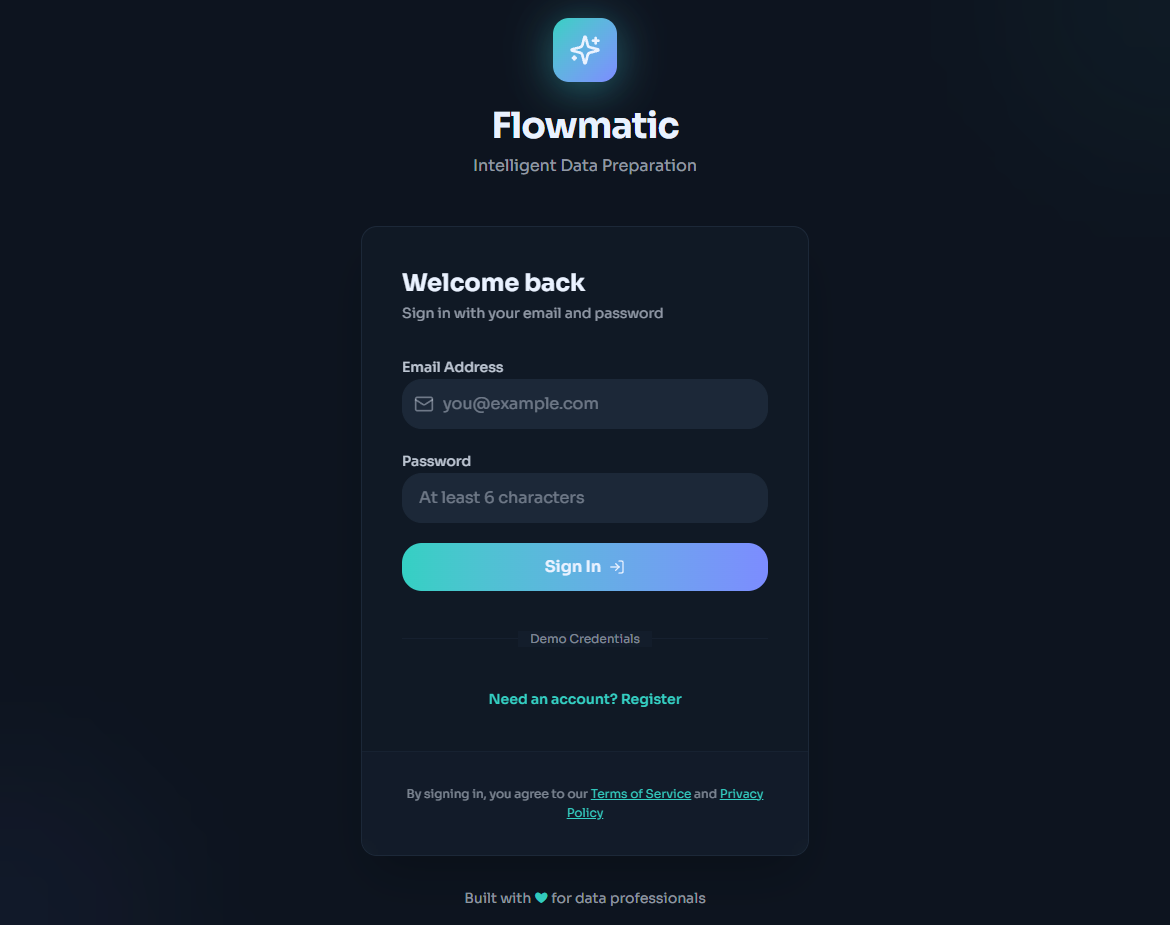
\includegraphics[width=0.55\textwidth]{figures/screenshots/00-login.png}
  \caption{Flowmatic login interface with organisation-scoped session authentication.}
  \label{fig:ui-login}
\end{figure}

\begin{figure}[H]
  \centering
  \begin{subfigure}[b]{0.48\textwidth}
    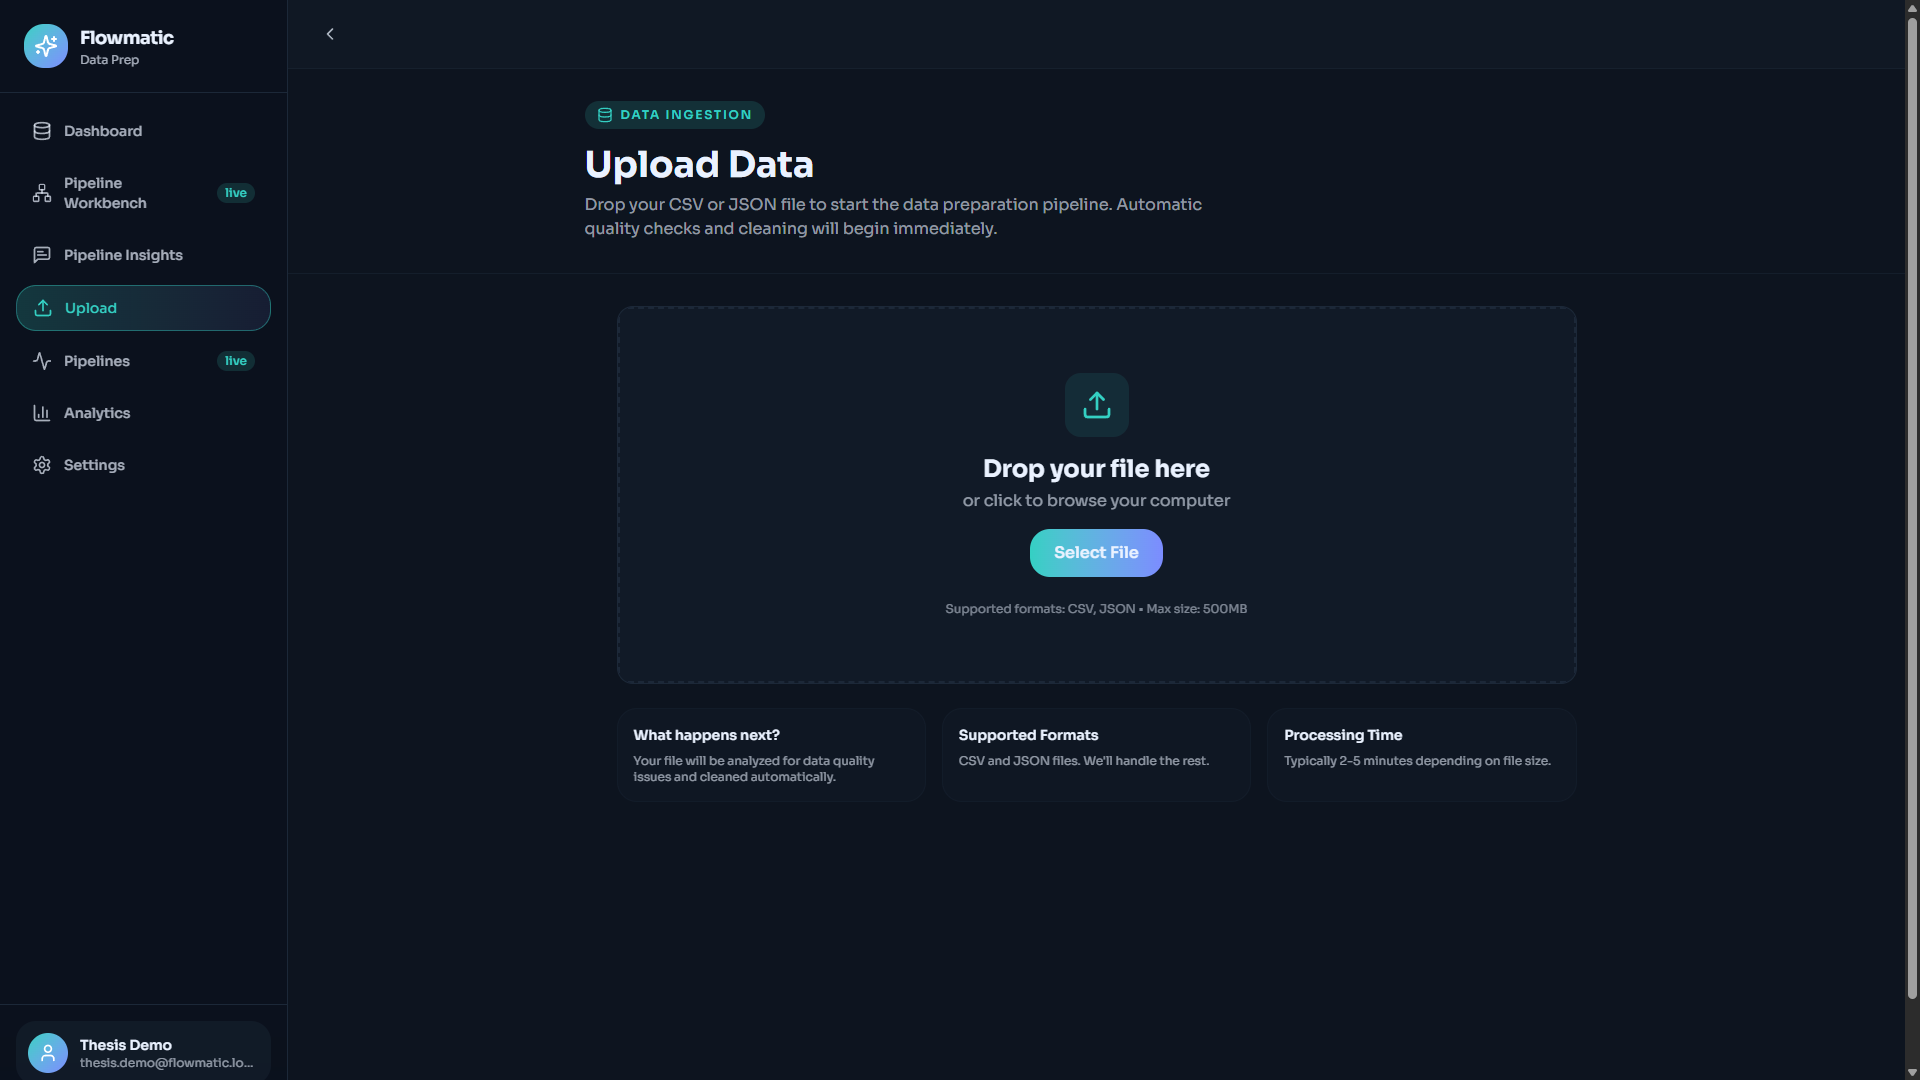
\includegraphics[width=\textwidth]{figures/screenshots/02-upload.png}
    \caption{Batch upload}
    \label{fig:ui-upload}
  \end{subfigure}\hfill
  \begin{subfigure}[b]{0.48\textwidth}
    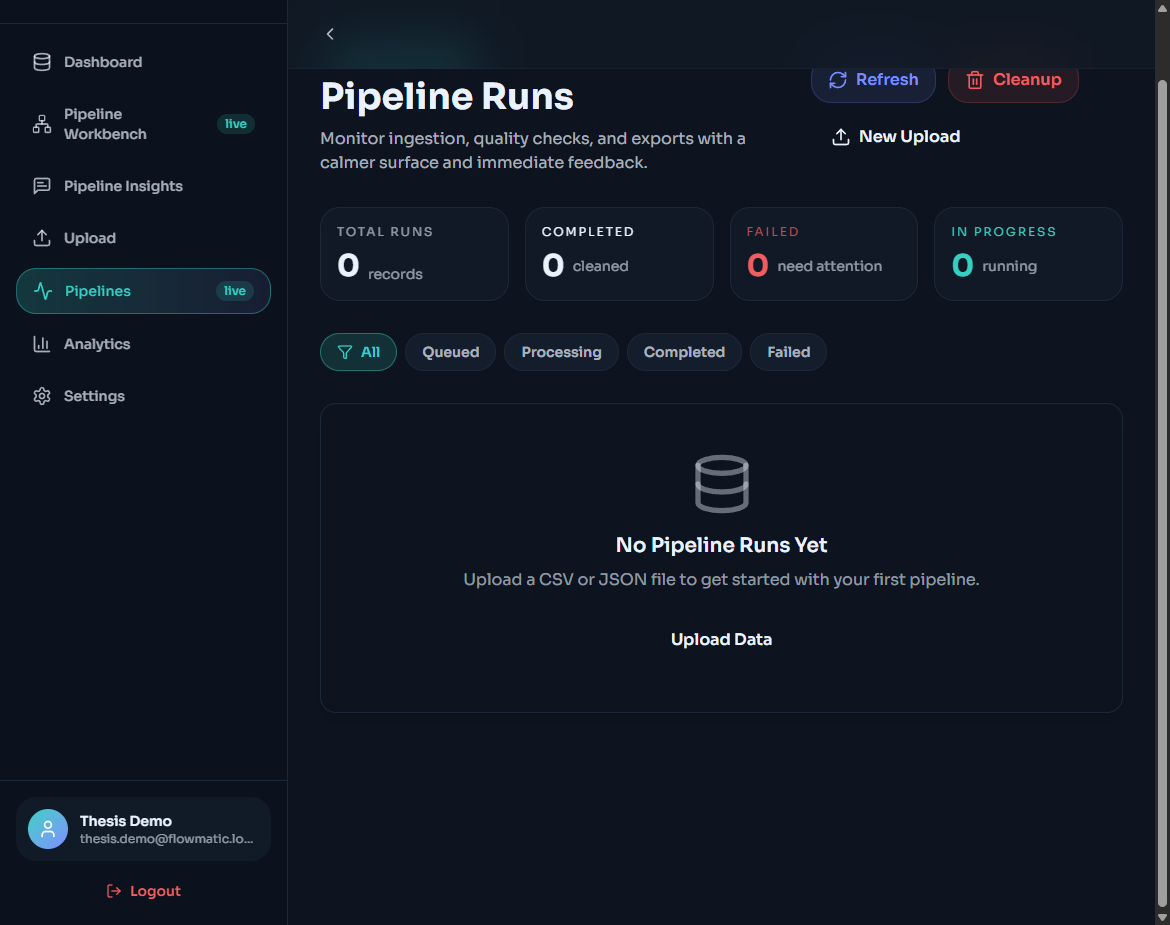
\includegraphics[width=\textwidth]{figures/screenshots/04-pipelines-runs.png}
    \caption{Pipeline runs}
    \label{fig:ui-pipelines}
  \end{subfigure}
  \caption{Tabular data preparation workflow: ingestion and run monitoring.}
  \label{fig:ui-batch-workflow}
\end{figure}

\begin{figure}[H]
  \centering
  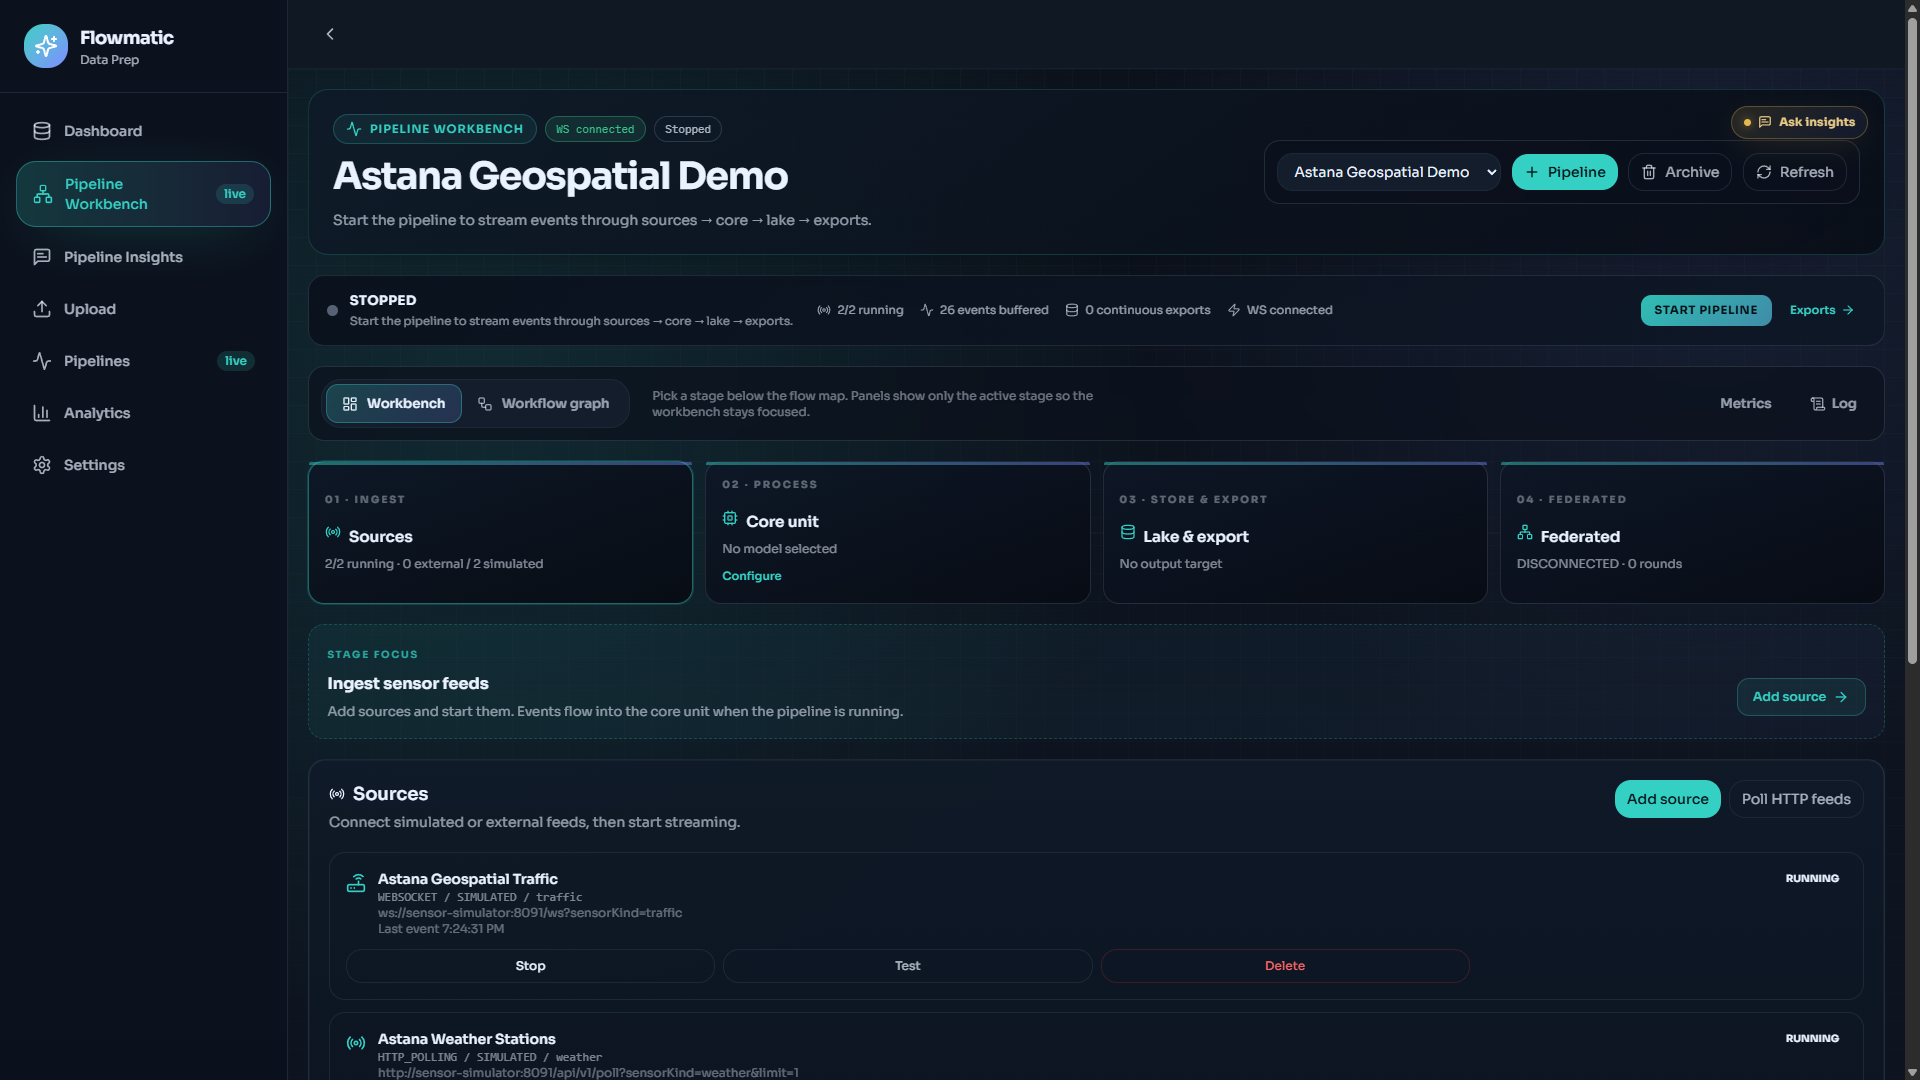
\includegraphics[width=0.92\textwidth]{figures/screenshots/08-smart-city-live-workbench.png}
  \caption{Astana Geospatial Demo workbench with simulated traffic (WebSocket) and weather sources, live event stream, and four-stage flow rail.}
  \label{fig:ui-smart-city-live}
\end{figure}

\begin{figure}[H]
  \centering
  \begin{subfigure}[b]{0.48\textwidth}
    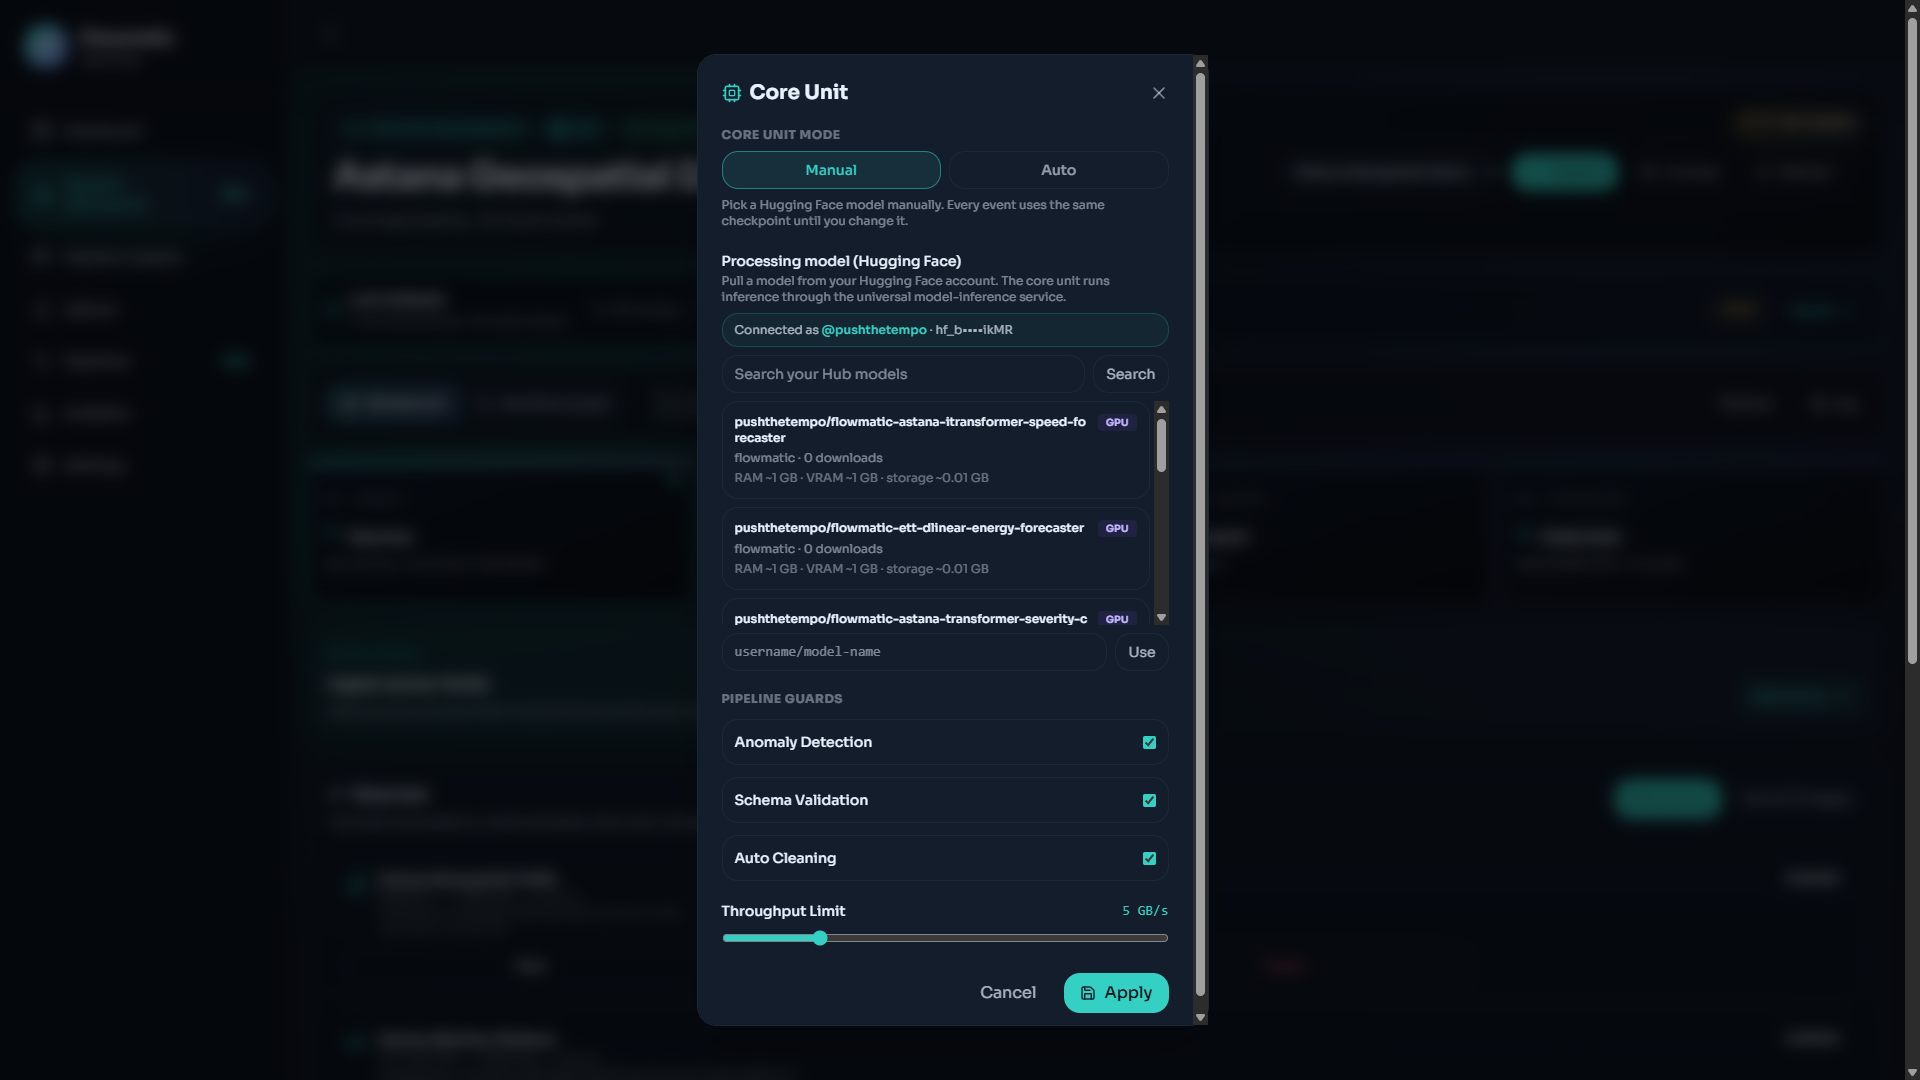
\includegraphics[width=\textwidth]{figures/screenshots/09-core-unit-huggingface-modal.png}
    \caption{Core unit configuration (Manual/Auto routing)}
    \label{fig:ui-core-unit}
  \end{subfigure}\hfill
  \begin{subfigure}[b]{0.48\textwidth}
    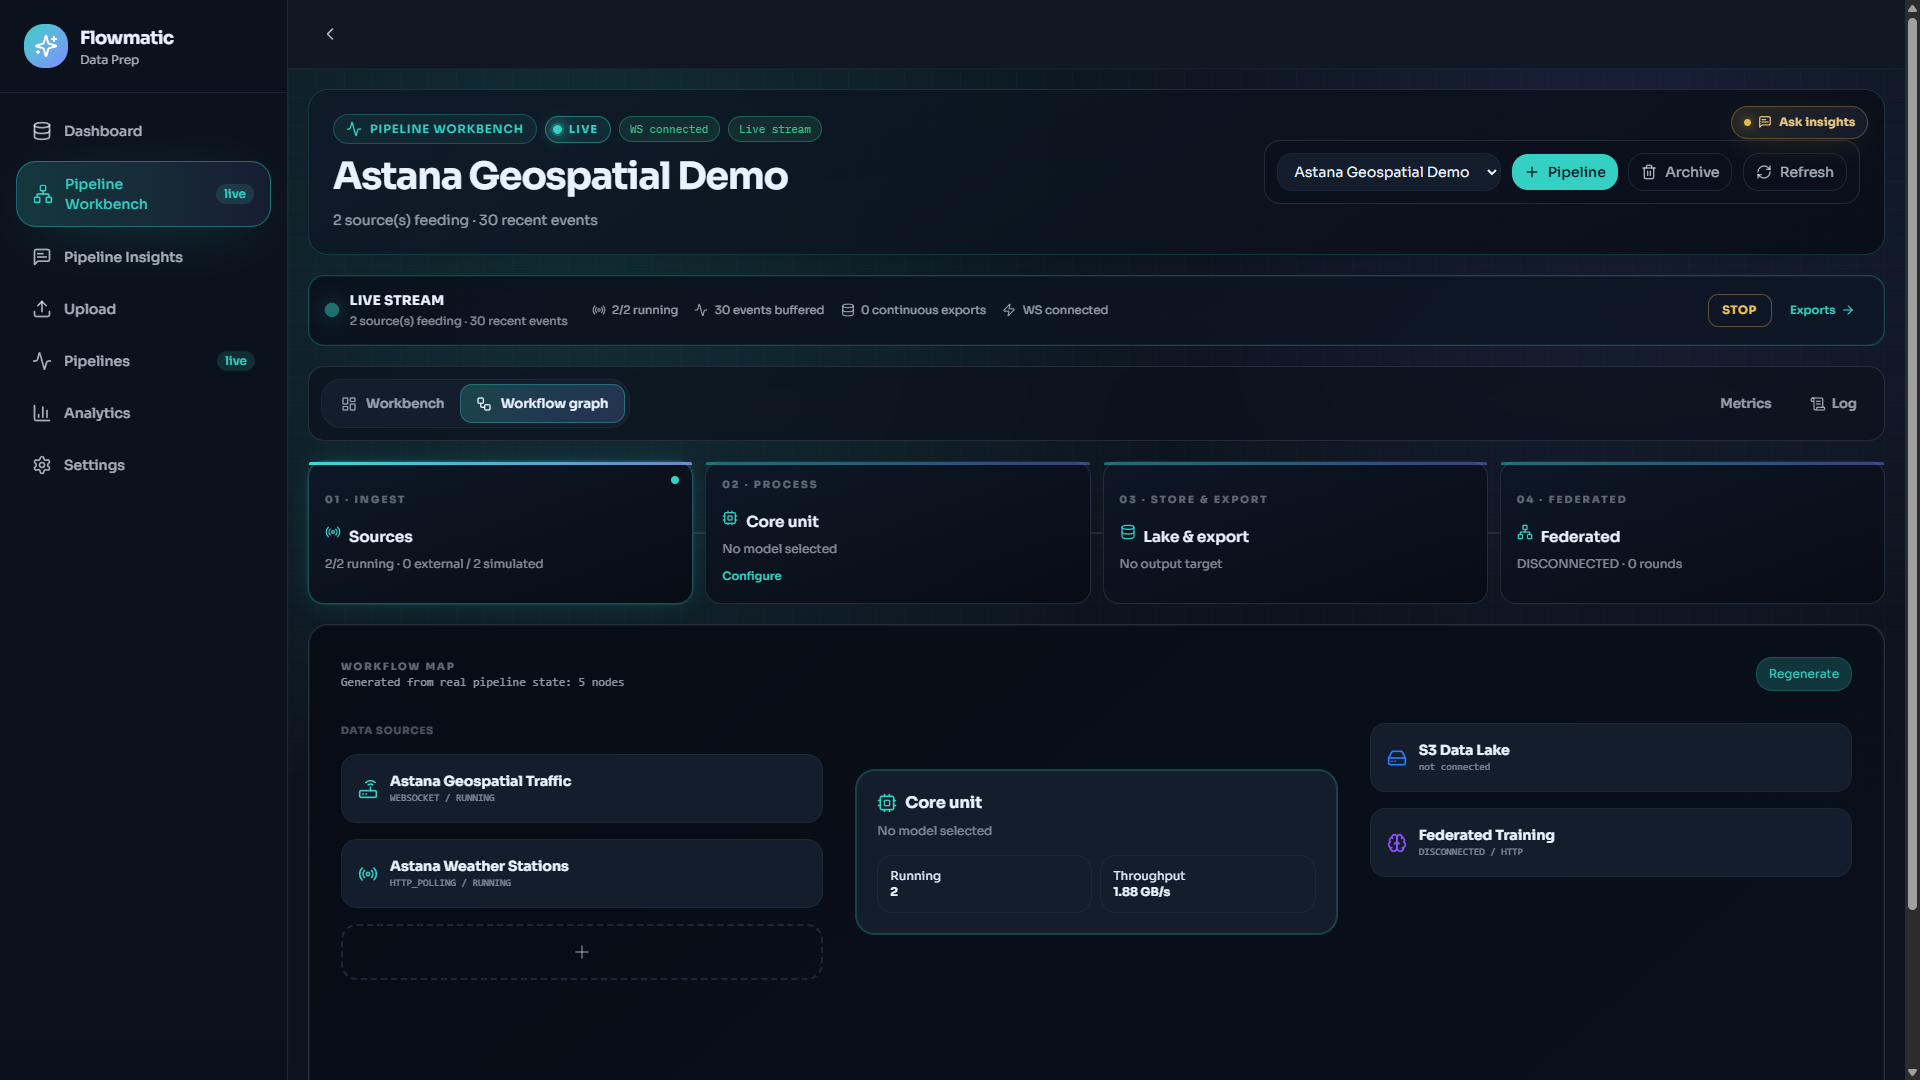
\includegraphics[width=\textwidth]{figures/screenshots/10-workflow-graph.png}
    \caption{Workflow graph view}
    \label{fig:ui-workflow-graph}
  \end{subfigure}
  \caption{Adaptive core unit and pipeline topology for the Astana geospatial simulator demo.}
  \label{fig:ui-config-graph}
\end{figure}

\begin{figure}[H]
  \centering
  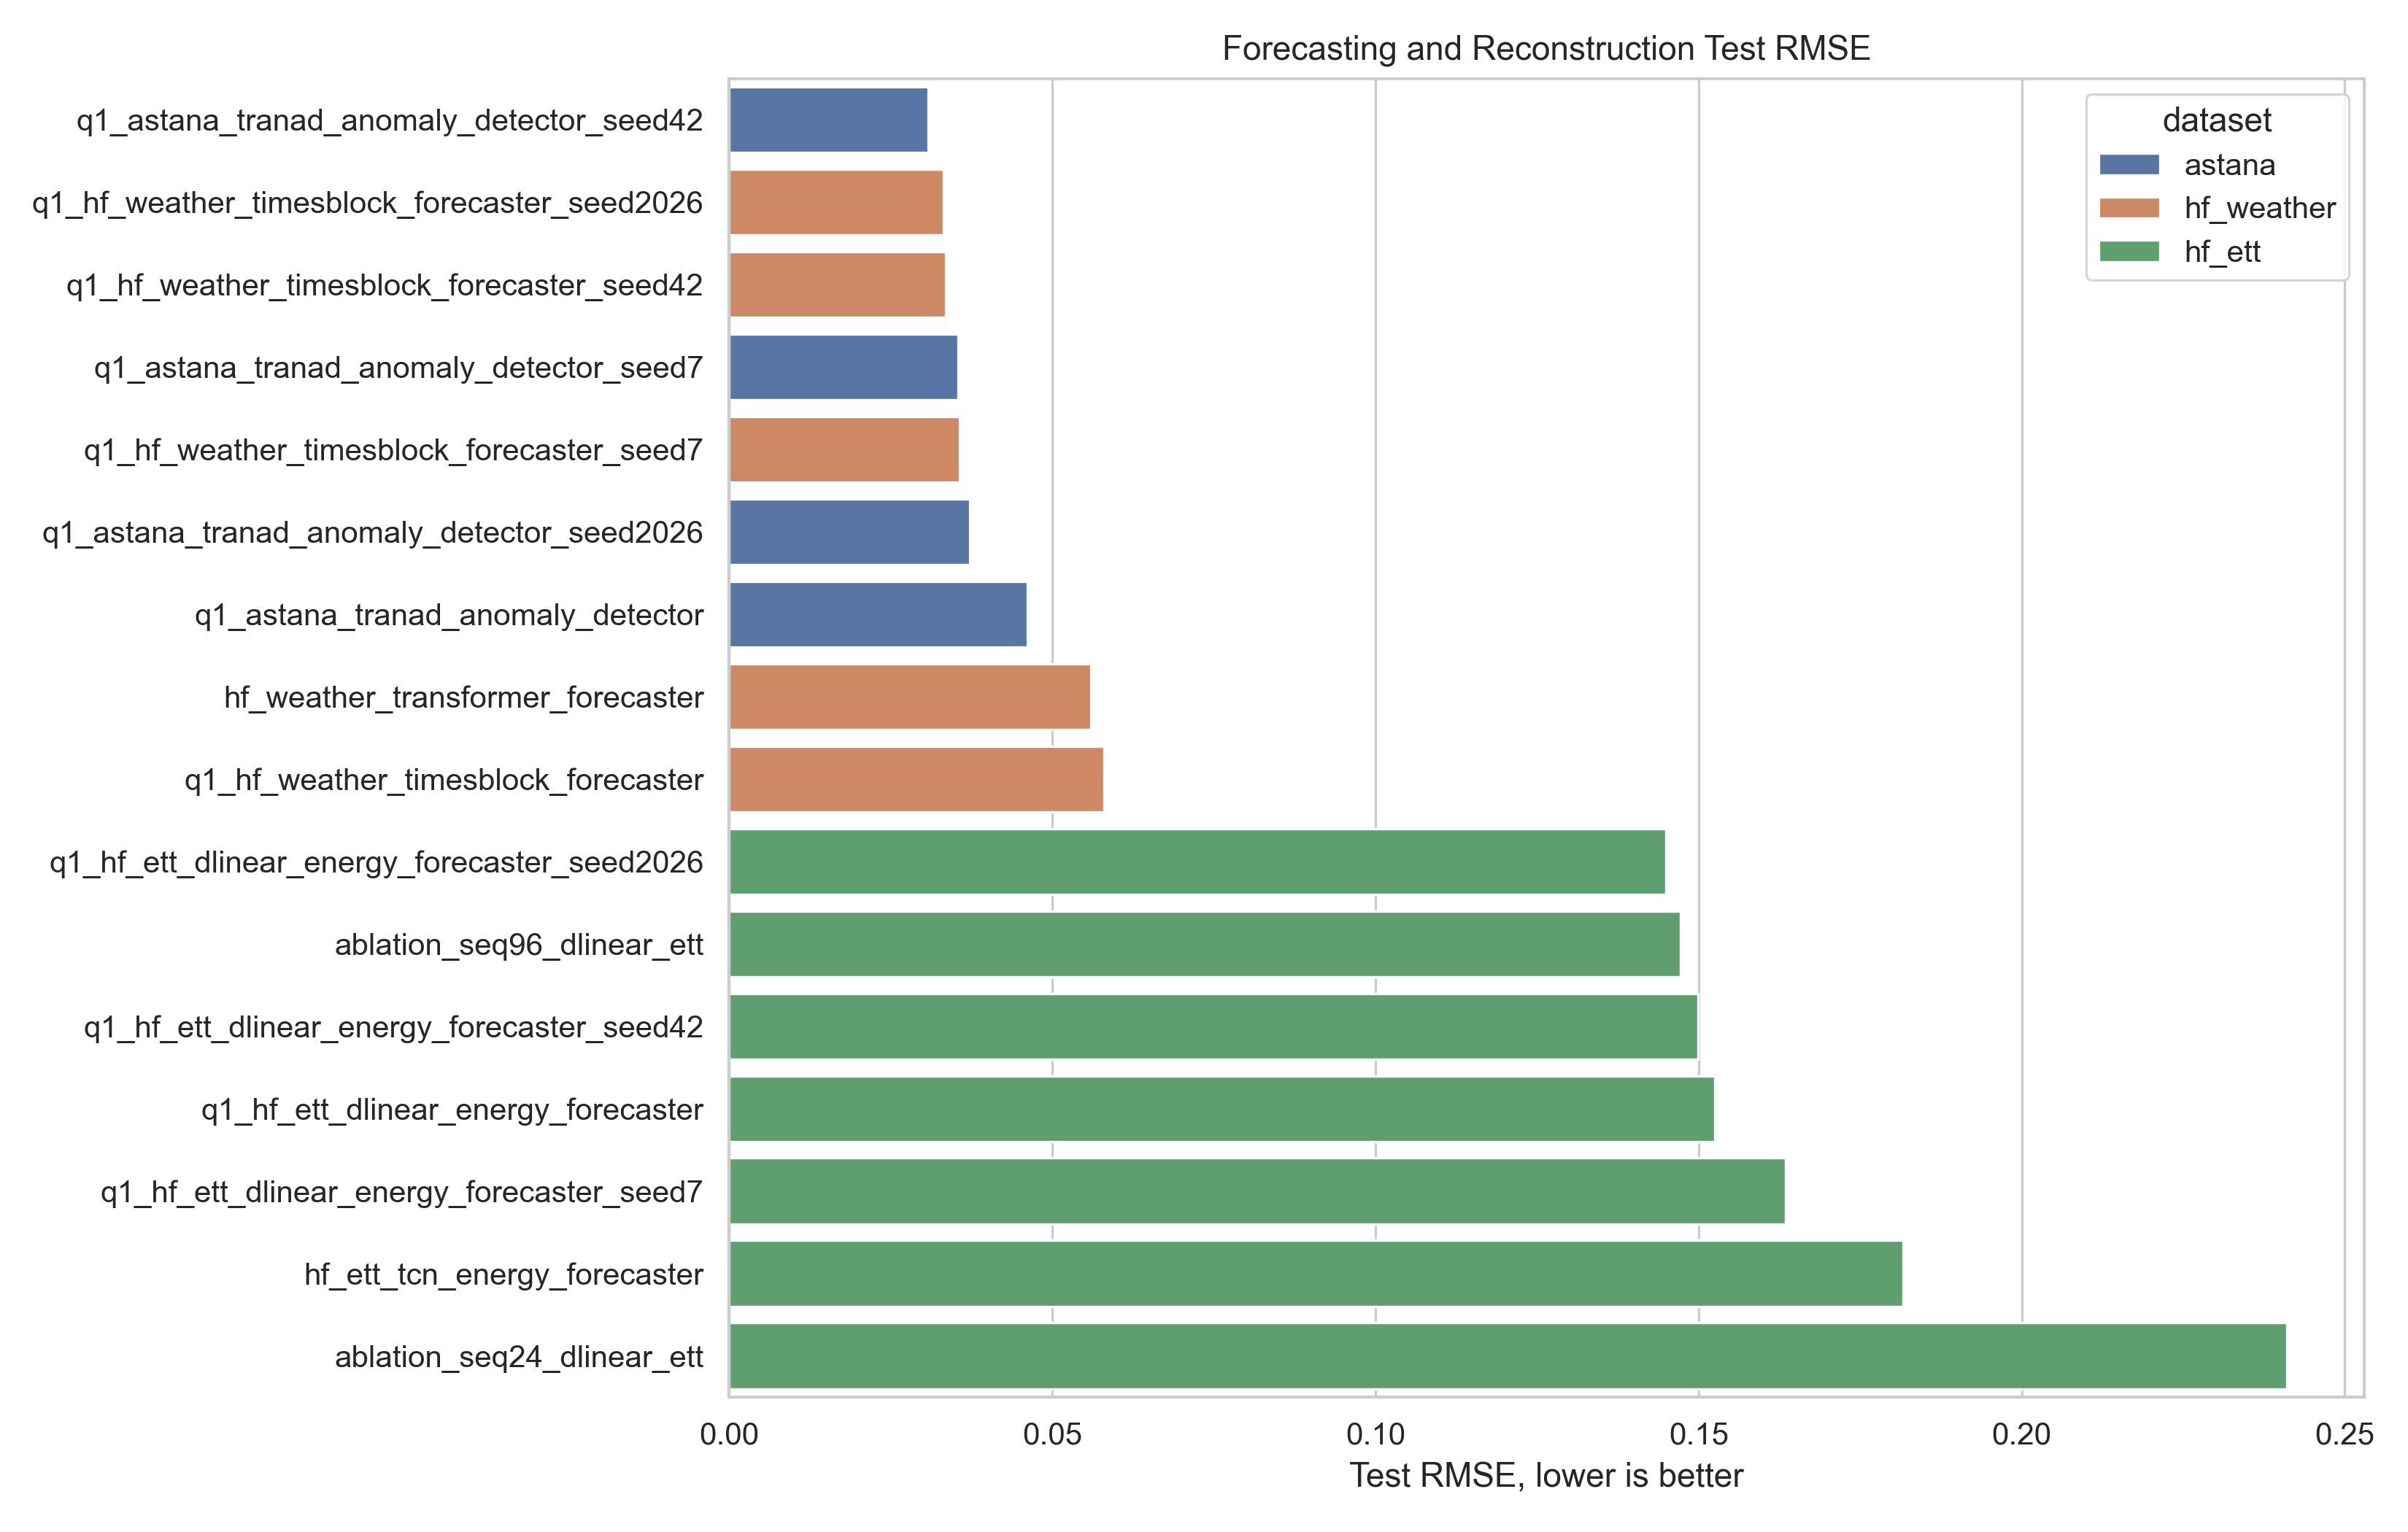
\includegraphics[width=0.85\textwidth]{figures/results/forecast_rmse_leaderboard.png}
  \caption{Forecasting and reconstruction leaderboard (test RMSE).}
  \label{fig:neural-forecast-rmse}
\end{figure}

\begin{figure}[H]
  \centering
  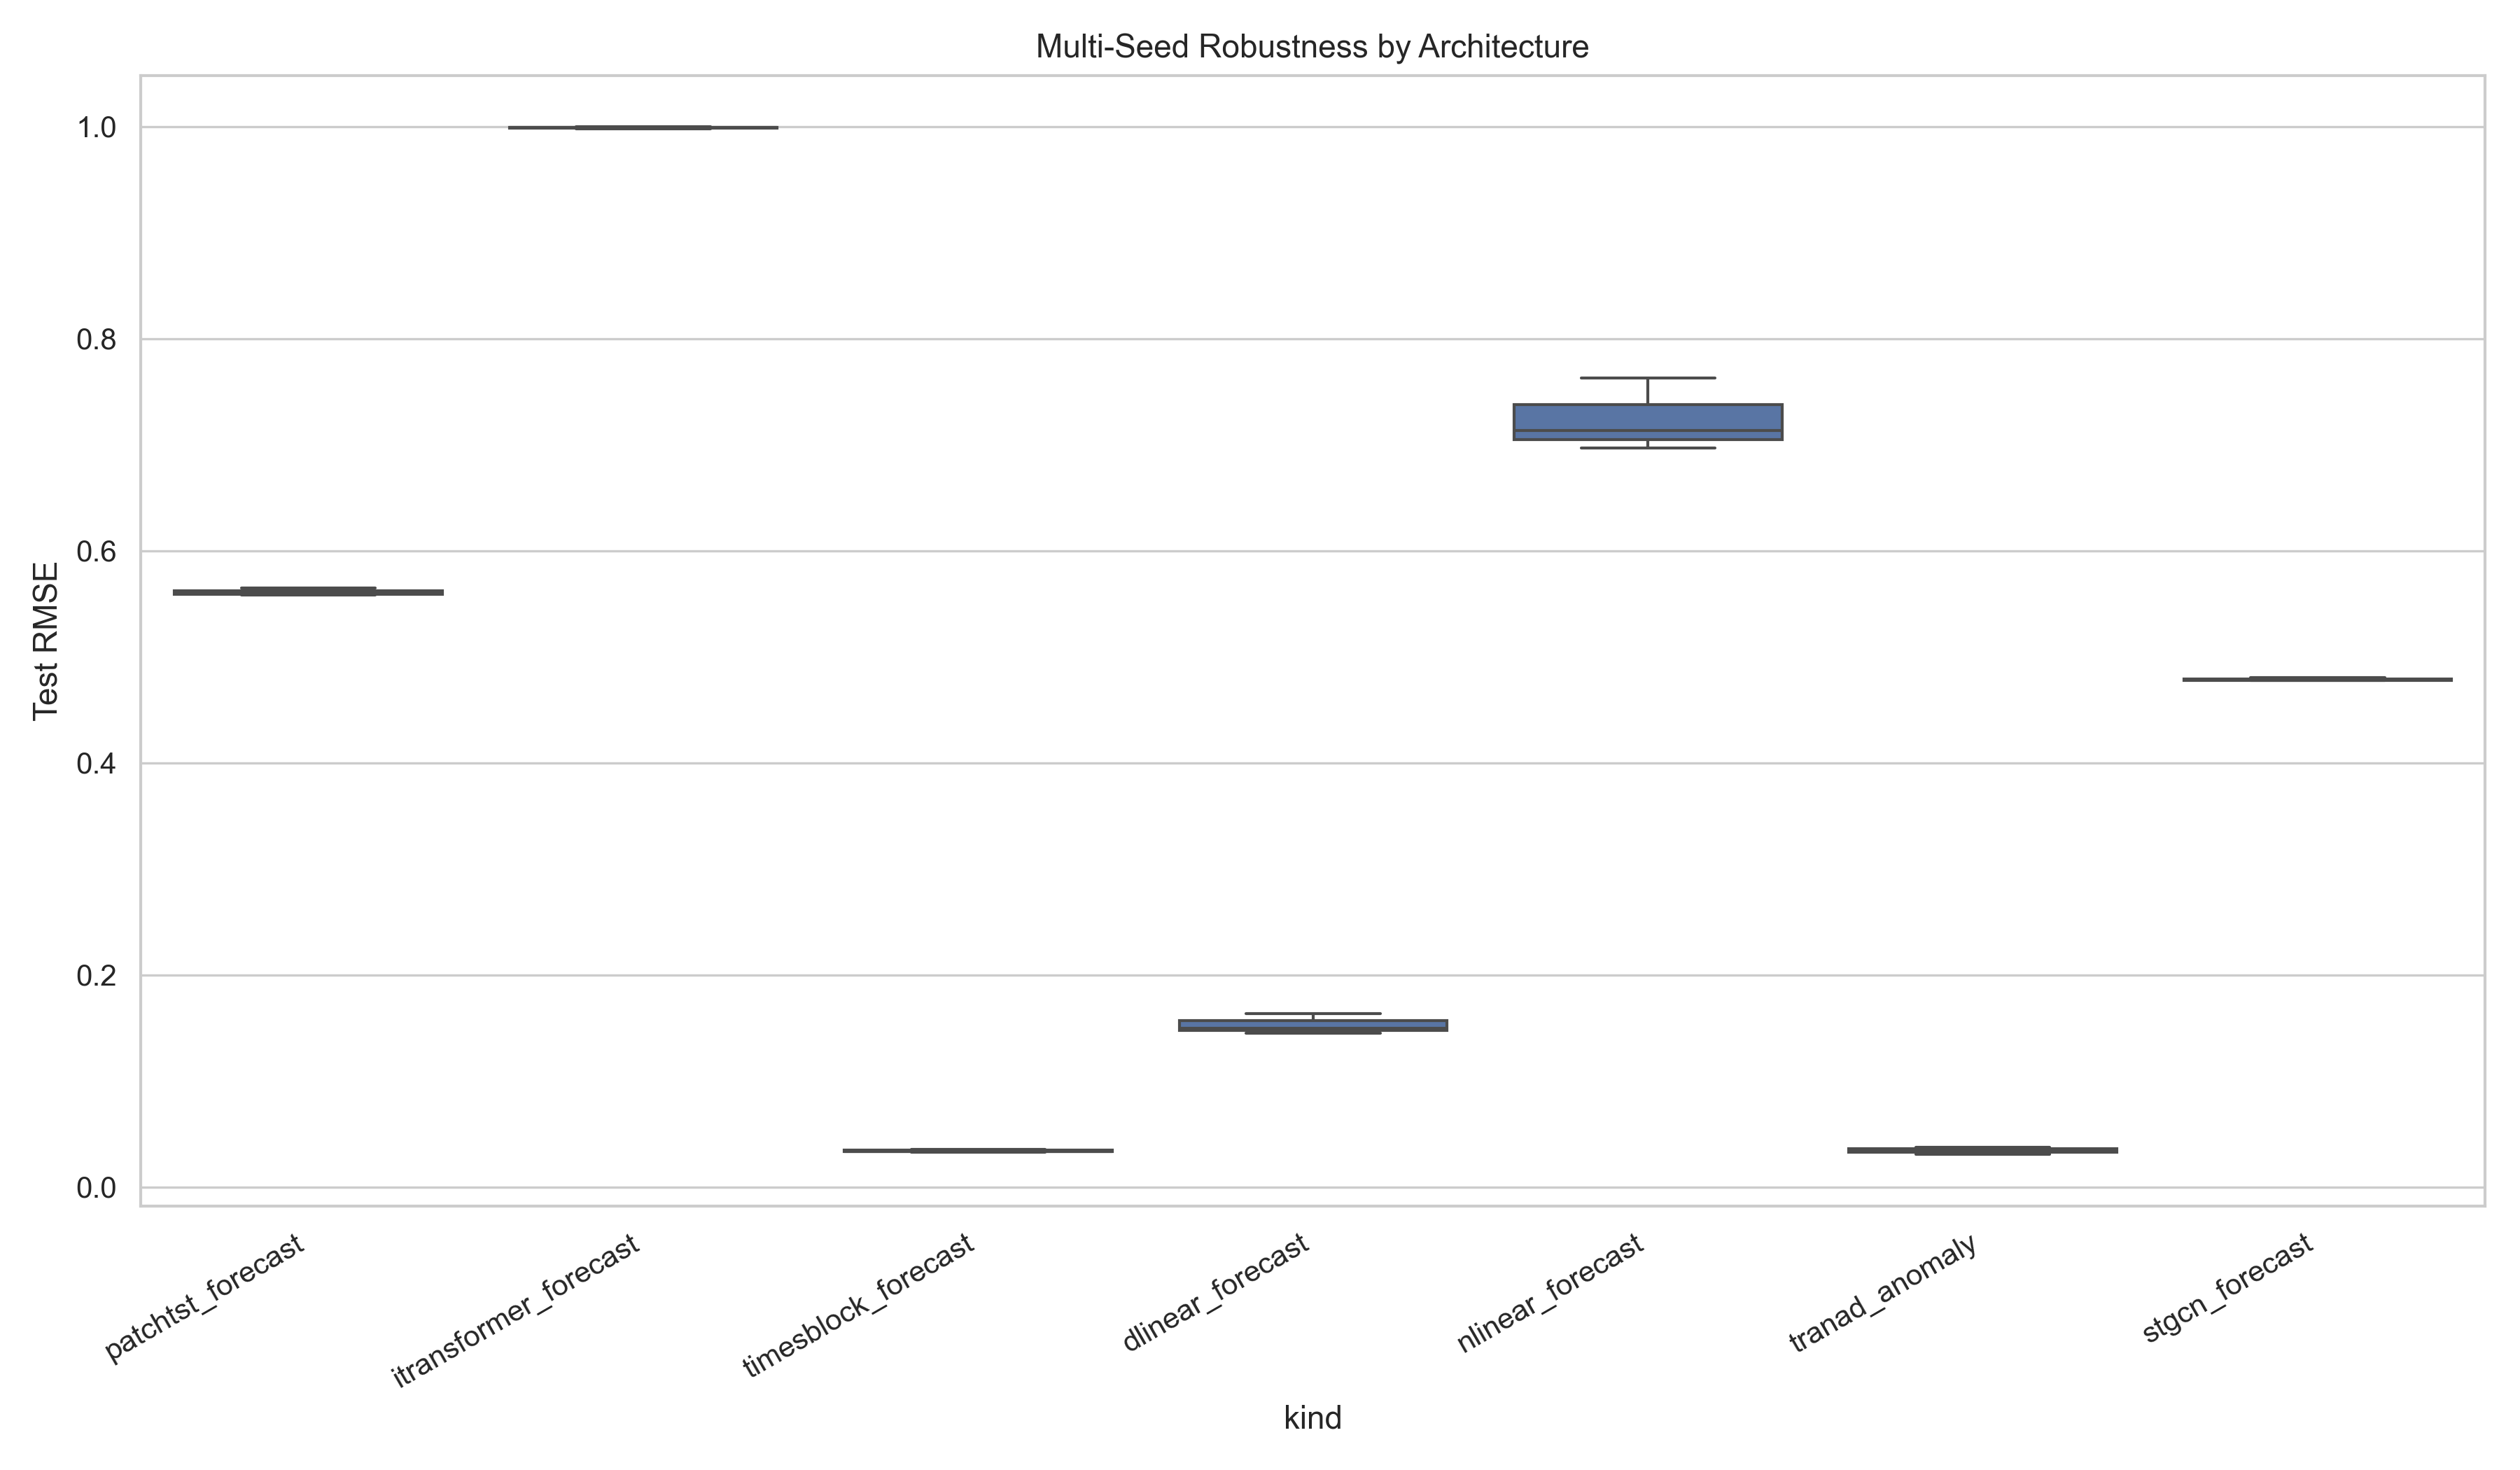
\includegraphics[width=0.85\textwidth]{figures/results/multi_seed_rmse_boxplot.png}
  \caption{Multi-seed test RMSE dispersion for production portfolio models.}
  \label{fig:neural-multiseed}
\end{figure}

\begin{figure}[H]
  \centering
  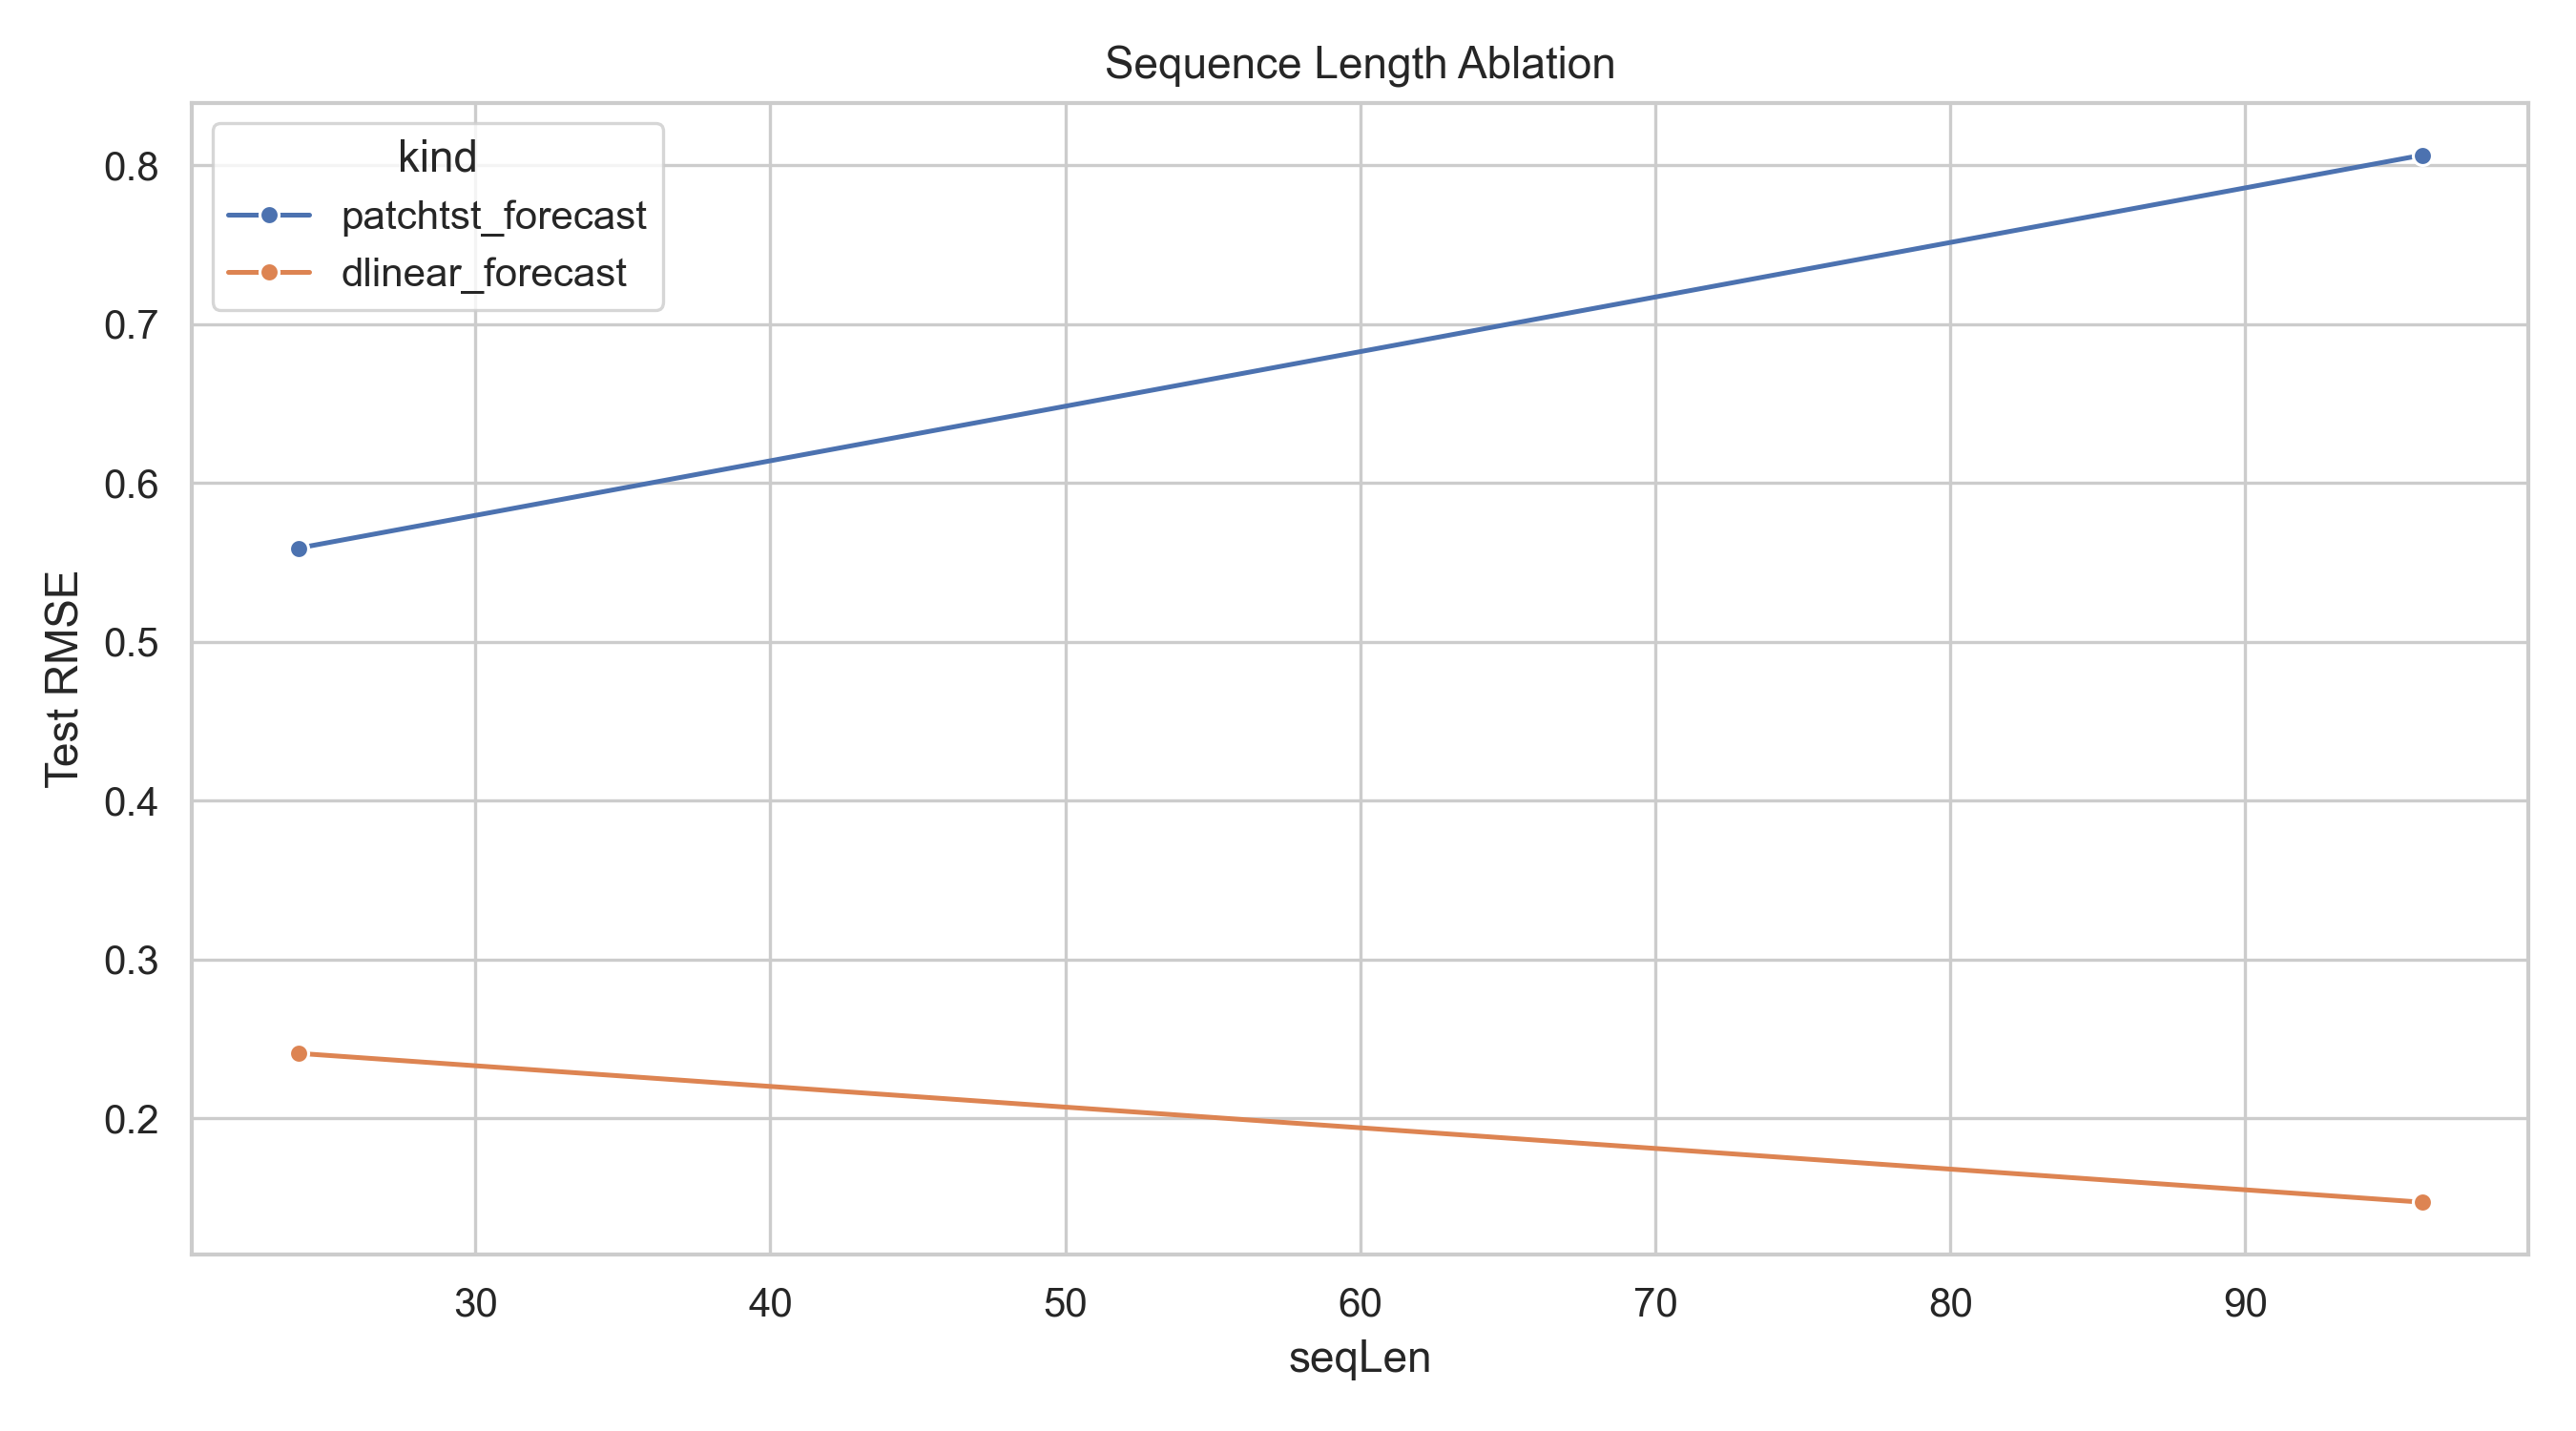
\includegraphics[width=0.78\textwidth]{figures/results/sequence_length_ablation.png}
  \caption{Sequence-length ablation ($L=24$ vs $L=96$).}
  \label{fig:seq-ablation}
\end{figure}

\begin{figure}[H]
  \centering
  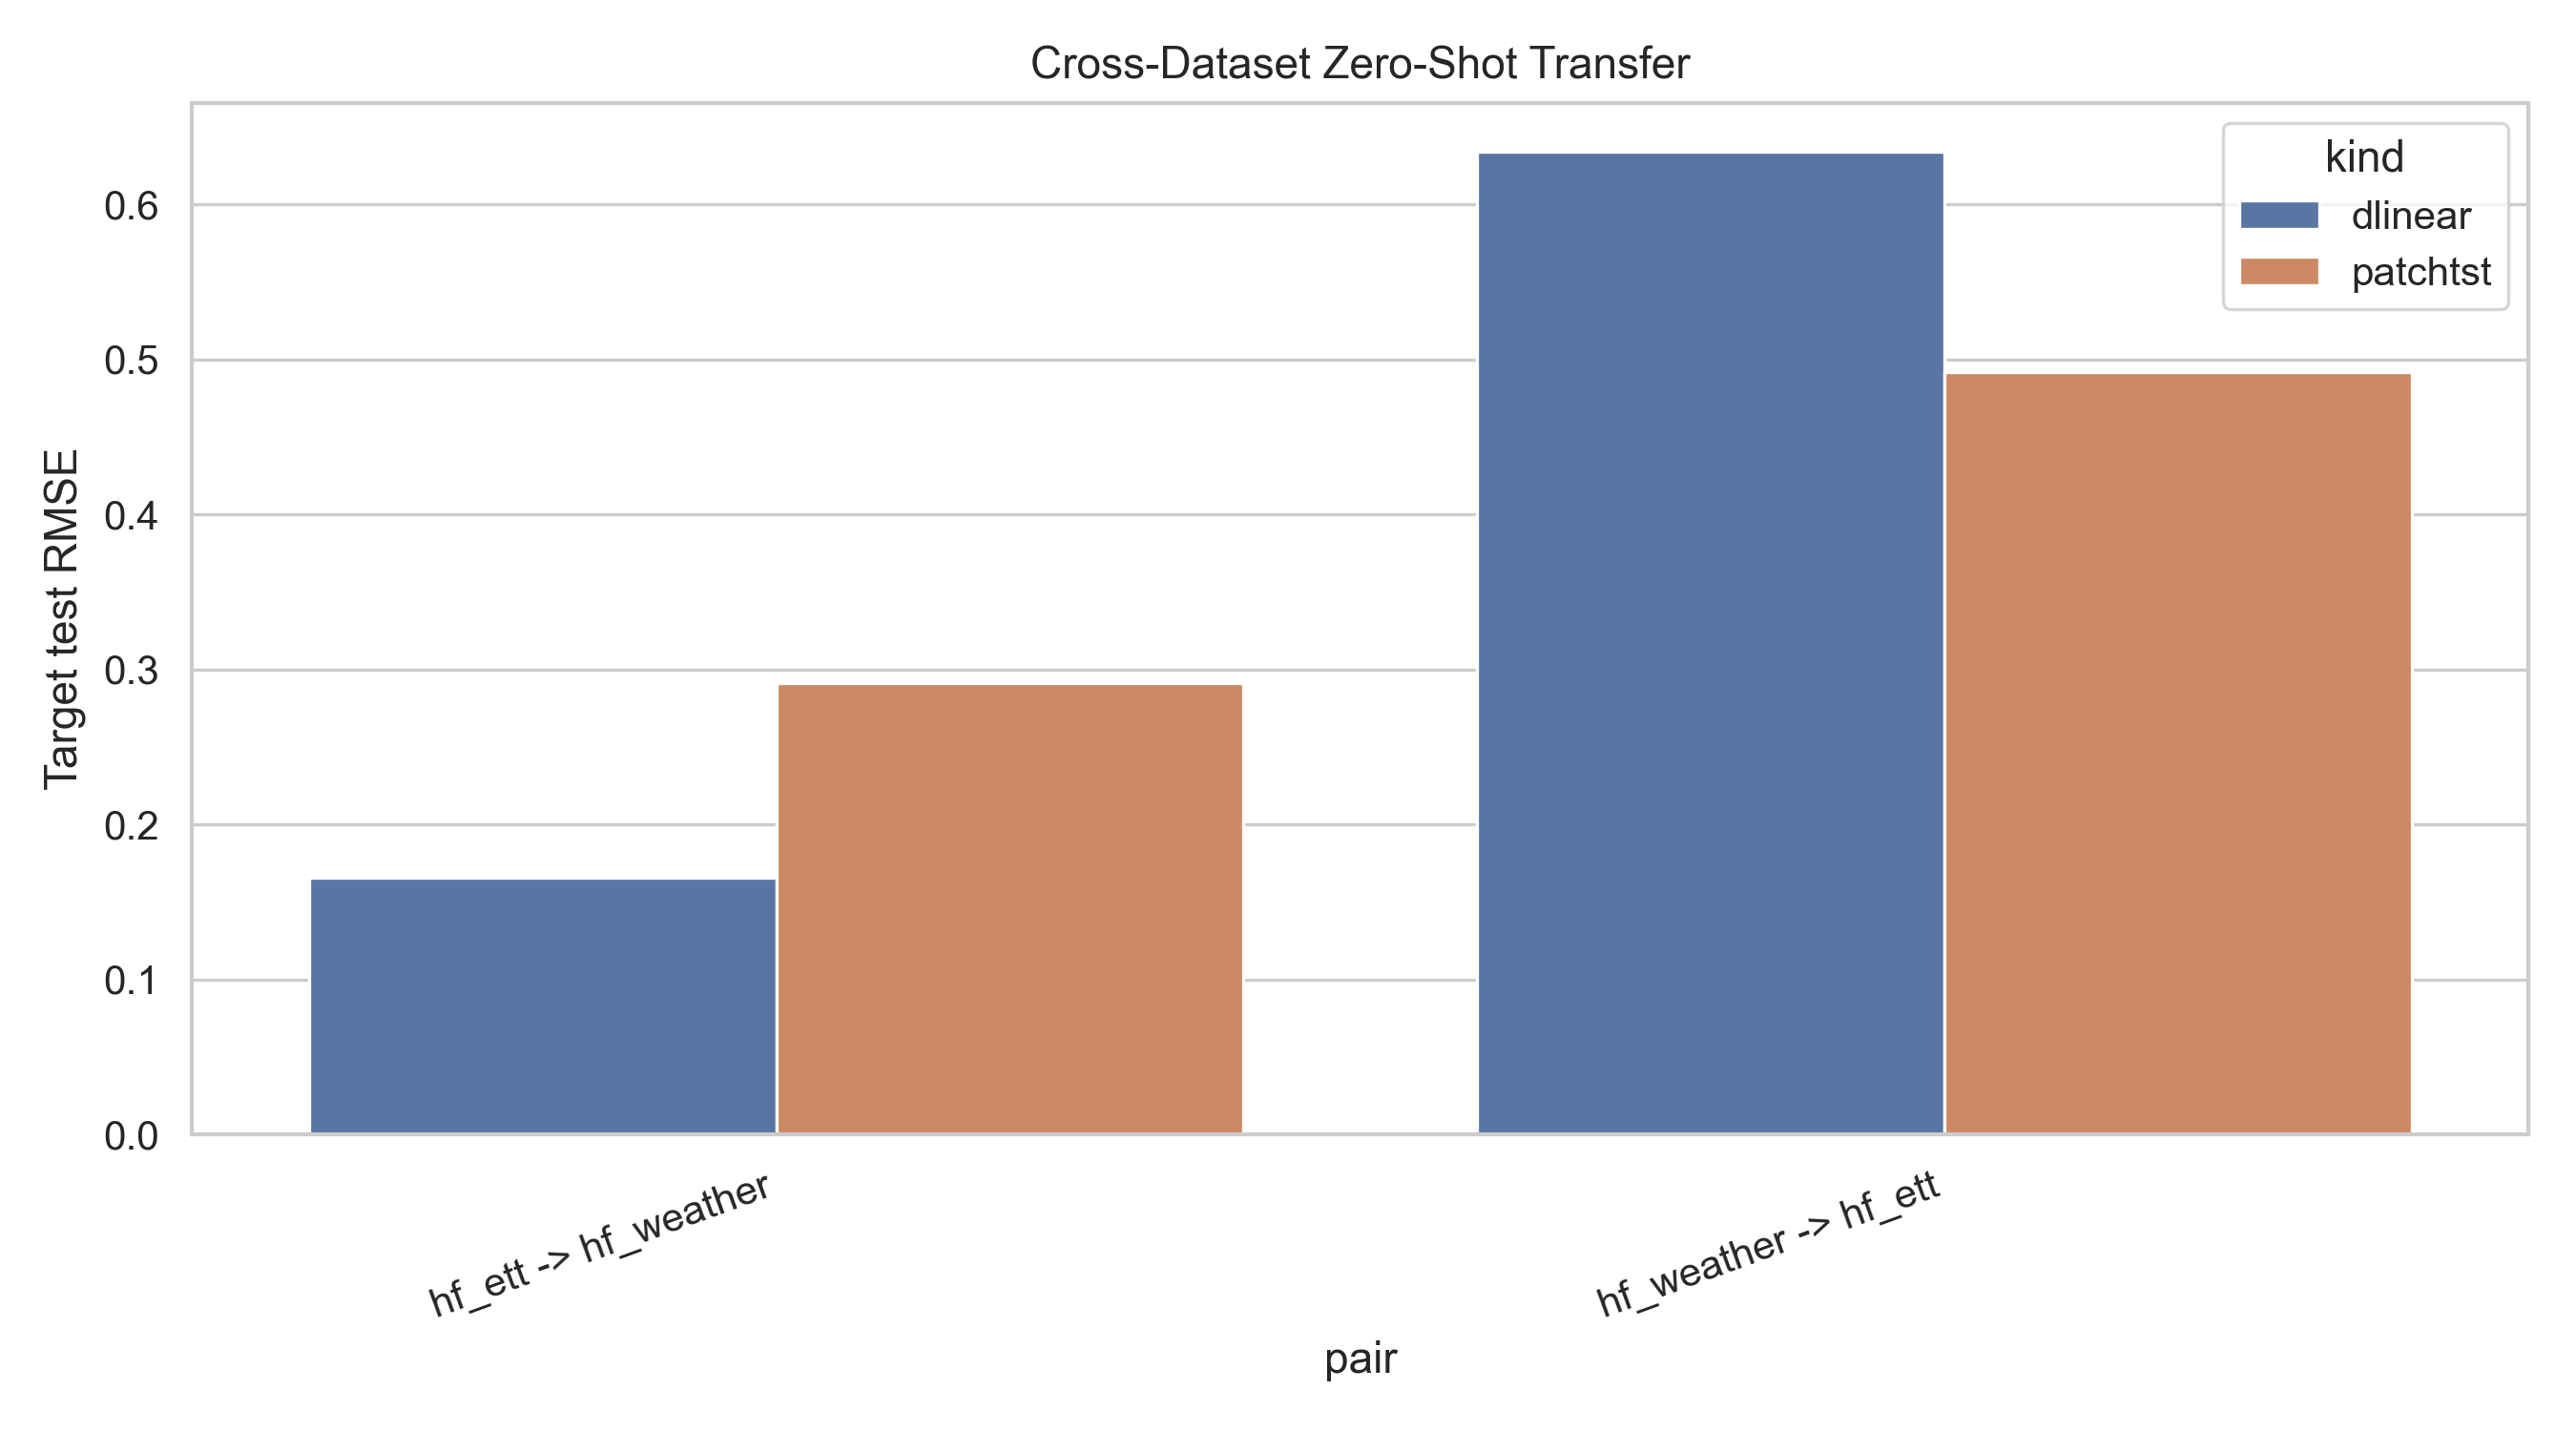
\includegraphics[width=0.78\textwidth]{figures/results/cross_dataset_transfer.png}
  \caption{Cross-dataset transfer (train source $\rightarrow$ test target).}
  \label{fig:cross-transfer}
\end{figure}

\begin{figure}[H]
  \centering
  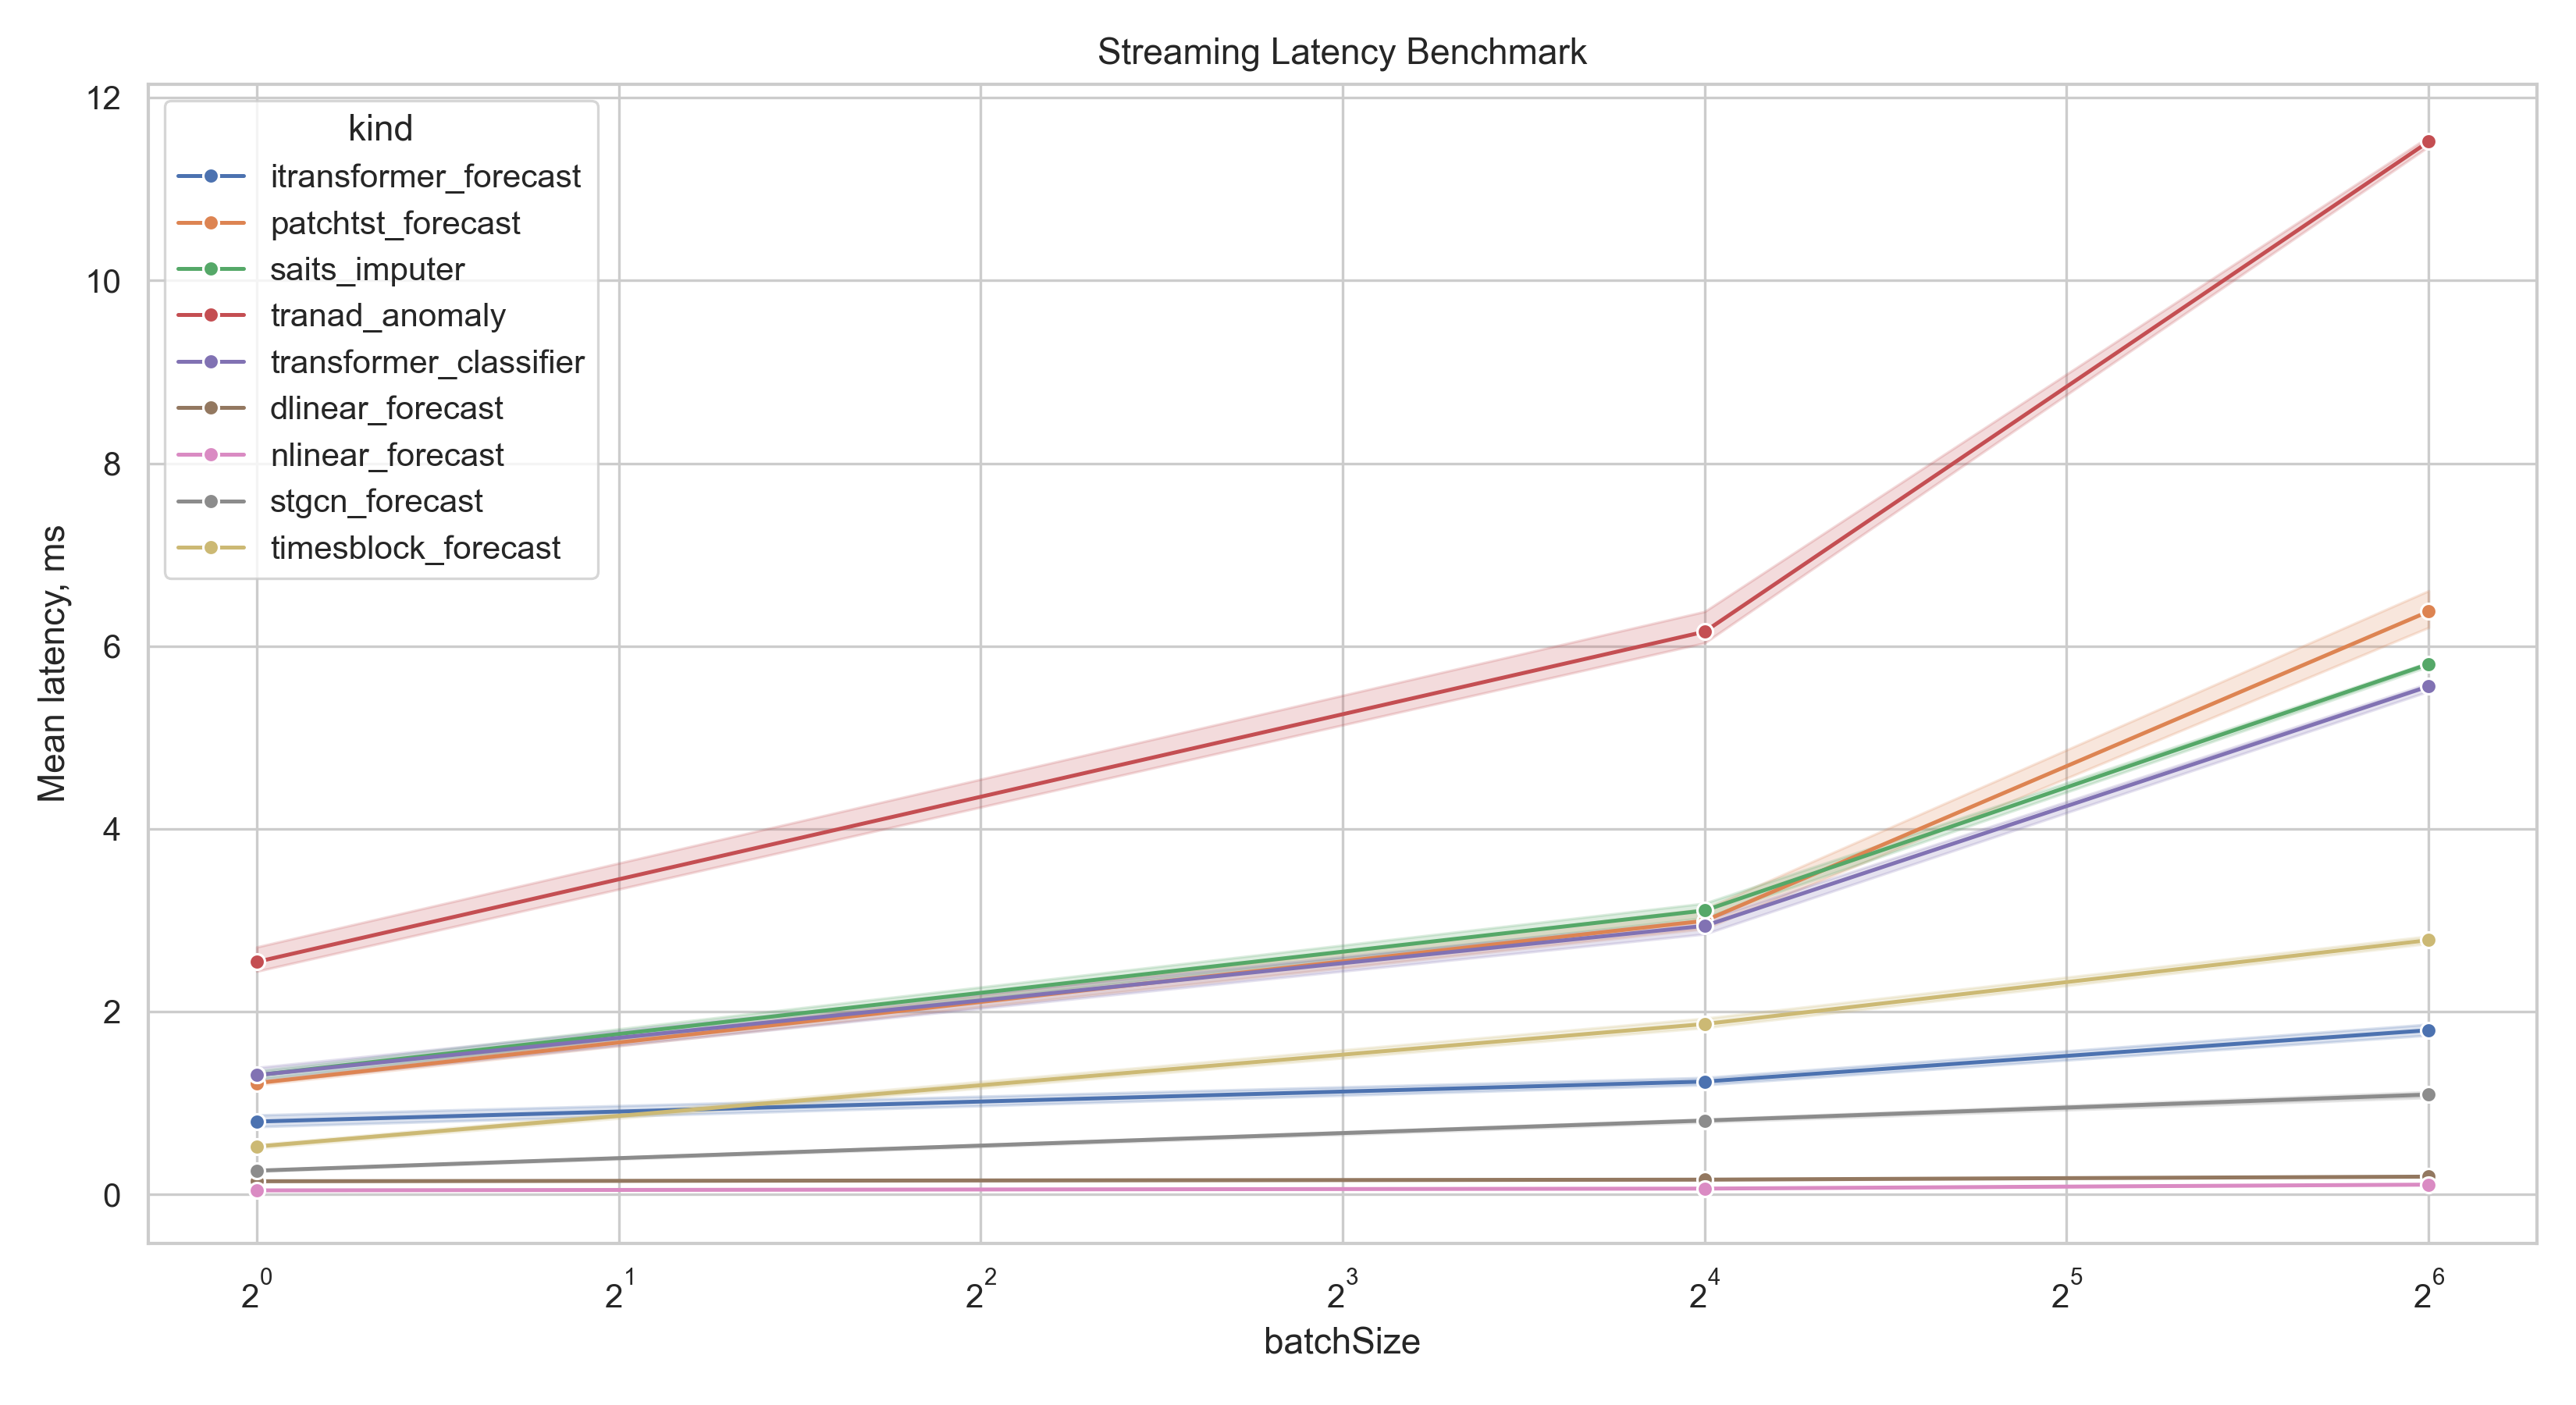
\includegraphics[width=0.78\textwidth]{figures/results/streaming_latency.png}
  \caption{Streaming inference latency vs batch size (TorchScript, GPU).}
  \label{fig:streaming-latency}
\end{figure}

\begin{figure}[H]
  \centering
  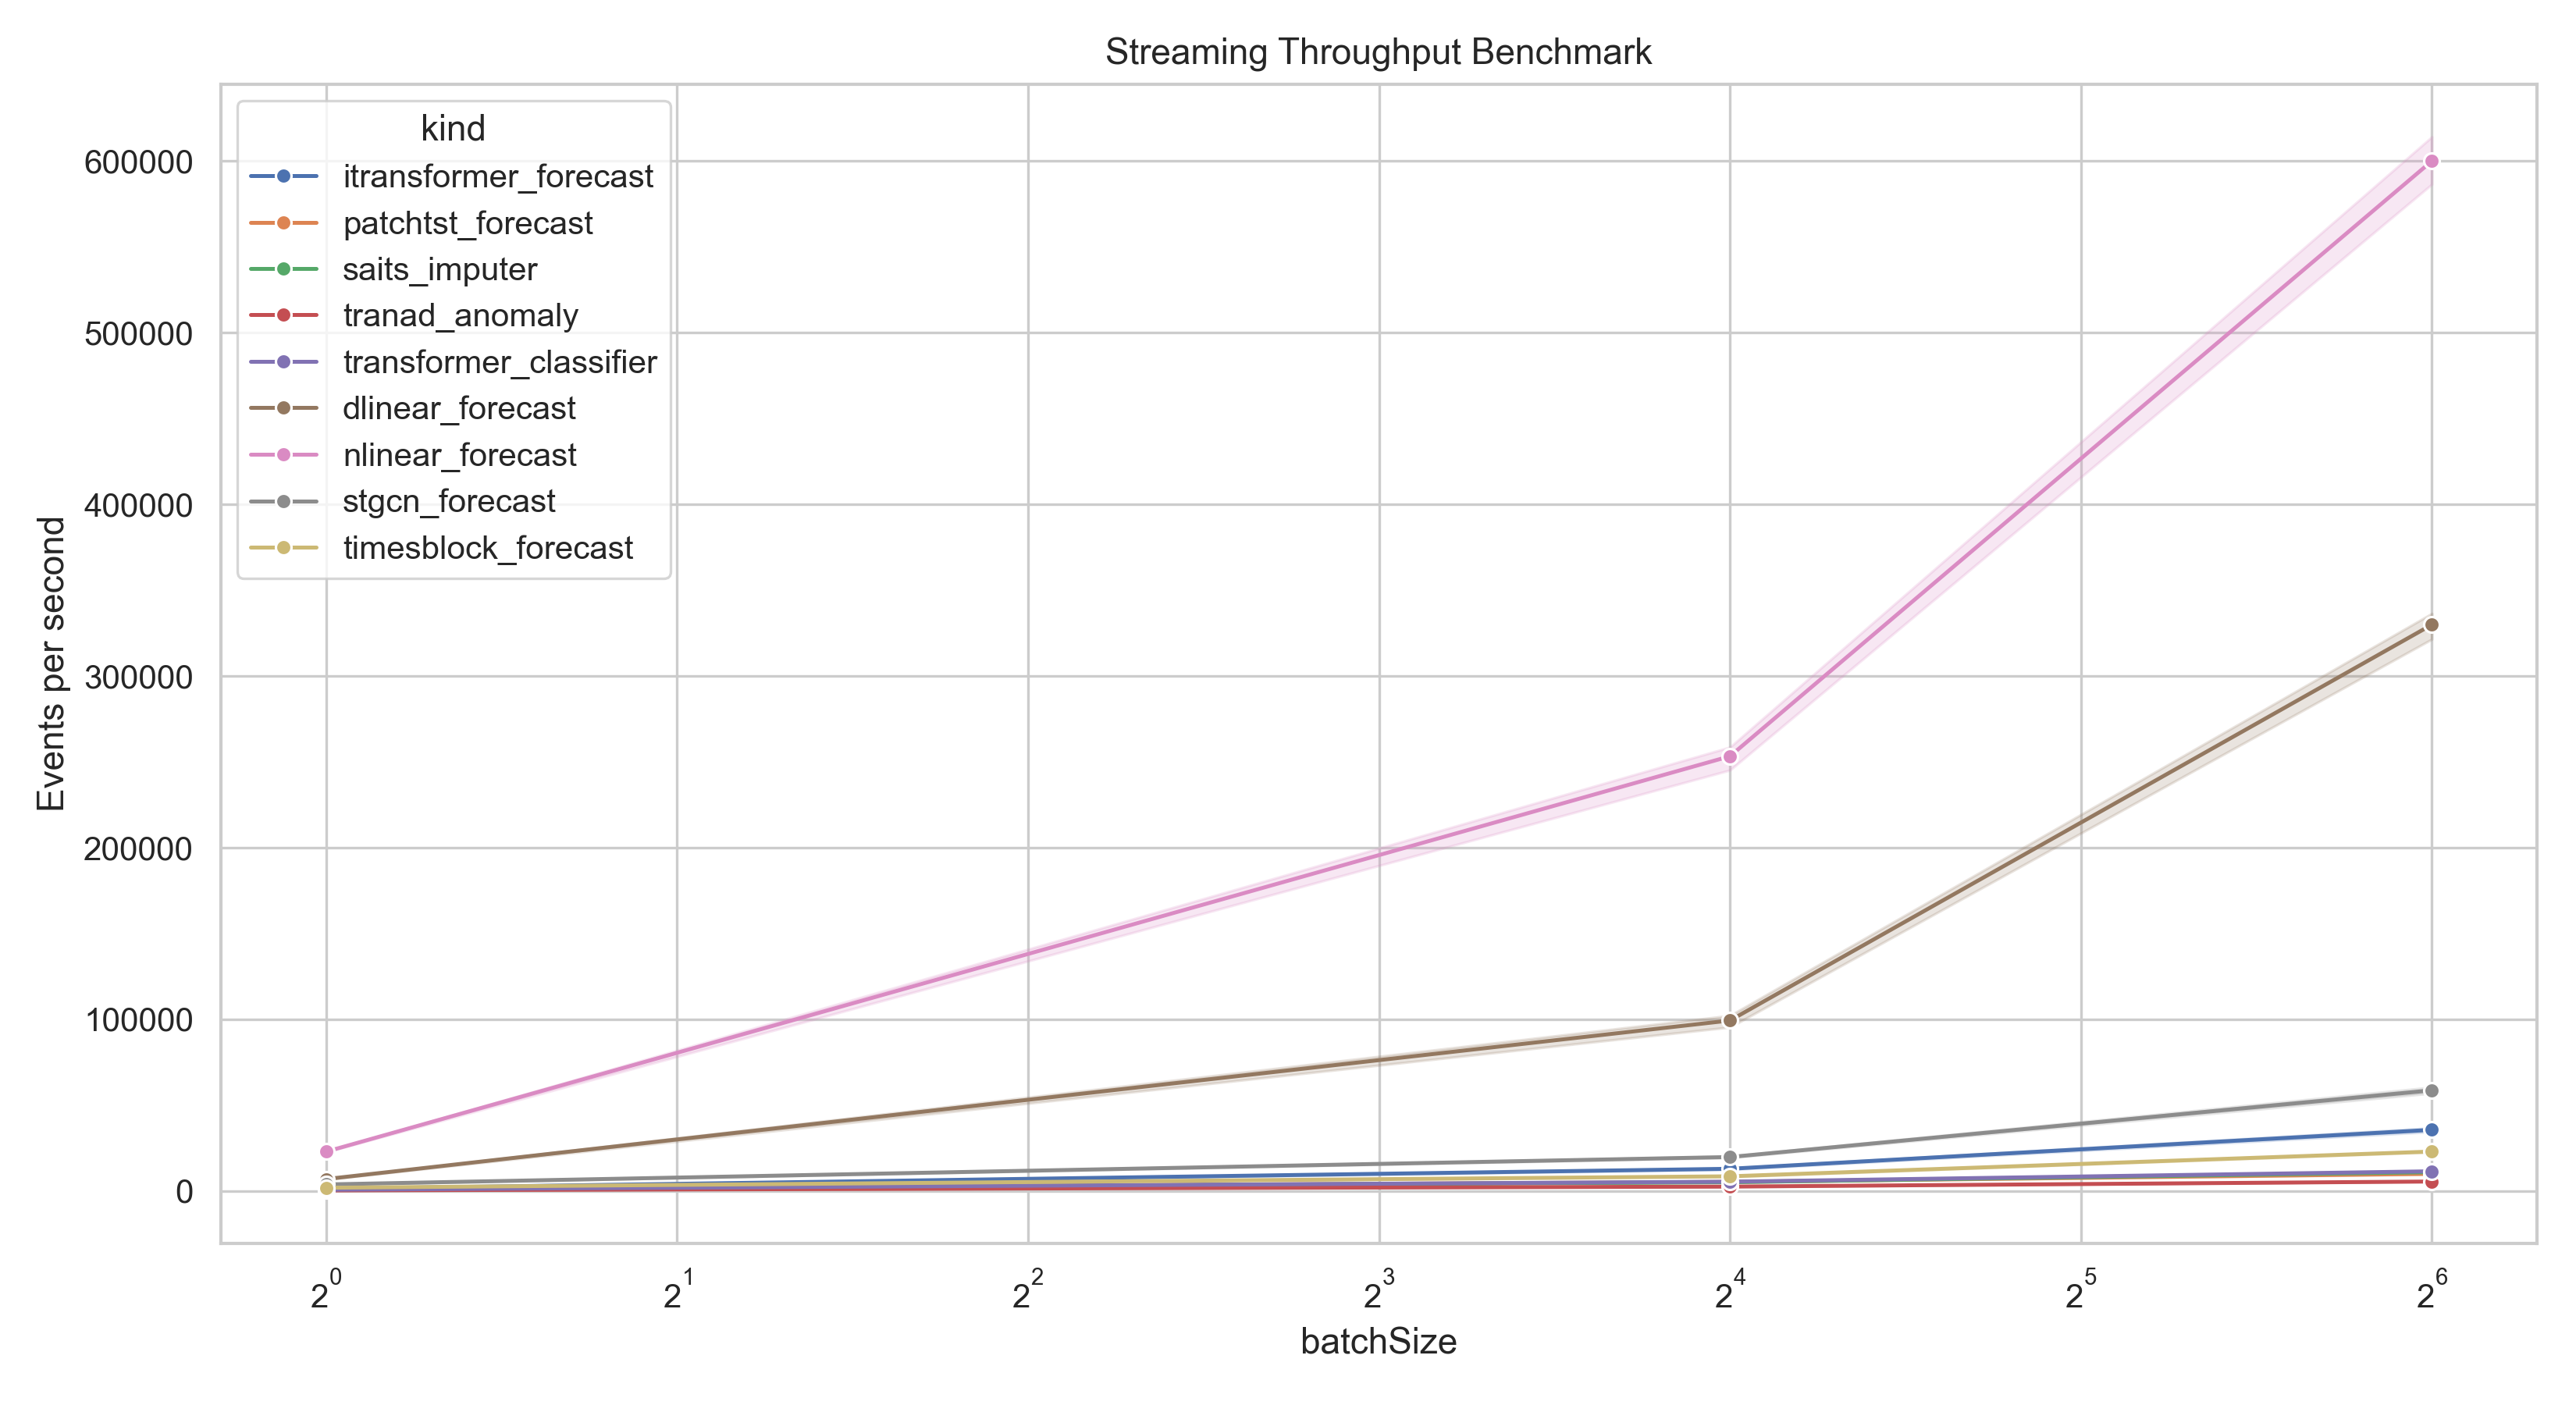
\includegraphics[width=0.78\textwidth]{figures/results/streaming_throughput.png}
  \caption{Streaming throughput (events/s) for production checkpoints.}
  \label{fig:streaming-throughput}
\end{figure}

\begin{figure}[H]
  \centering
  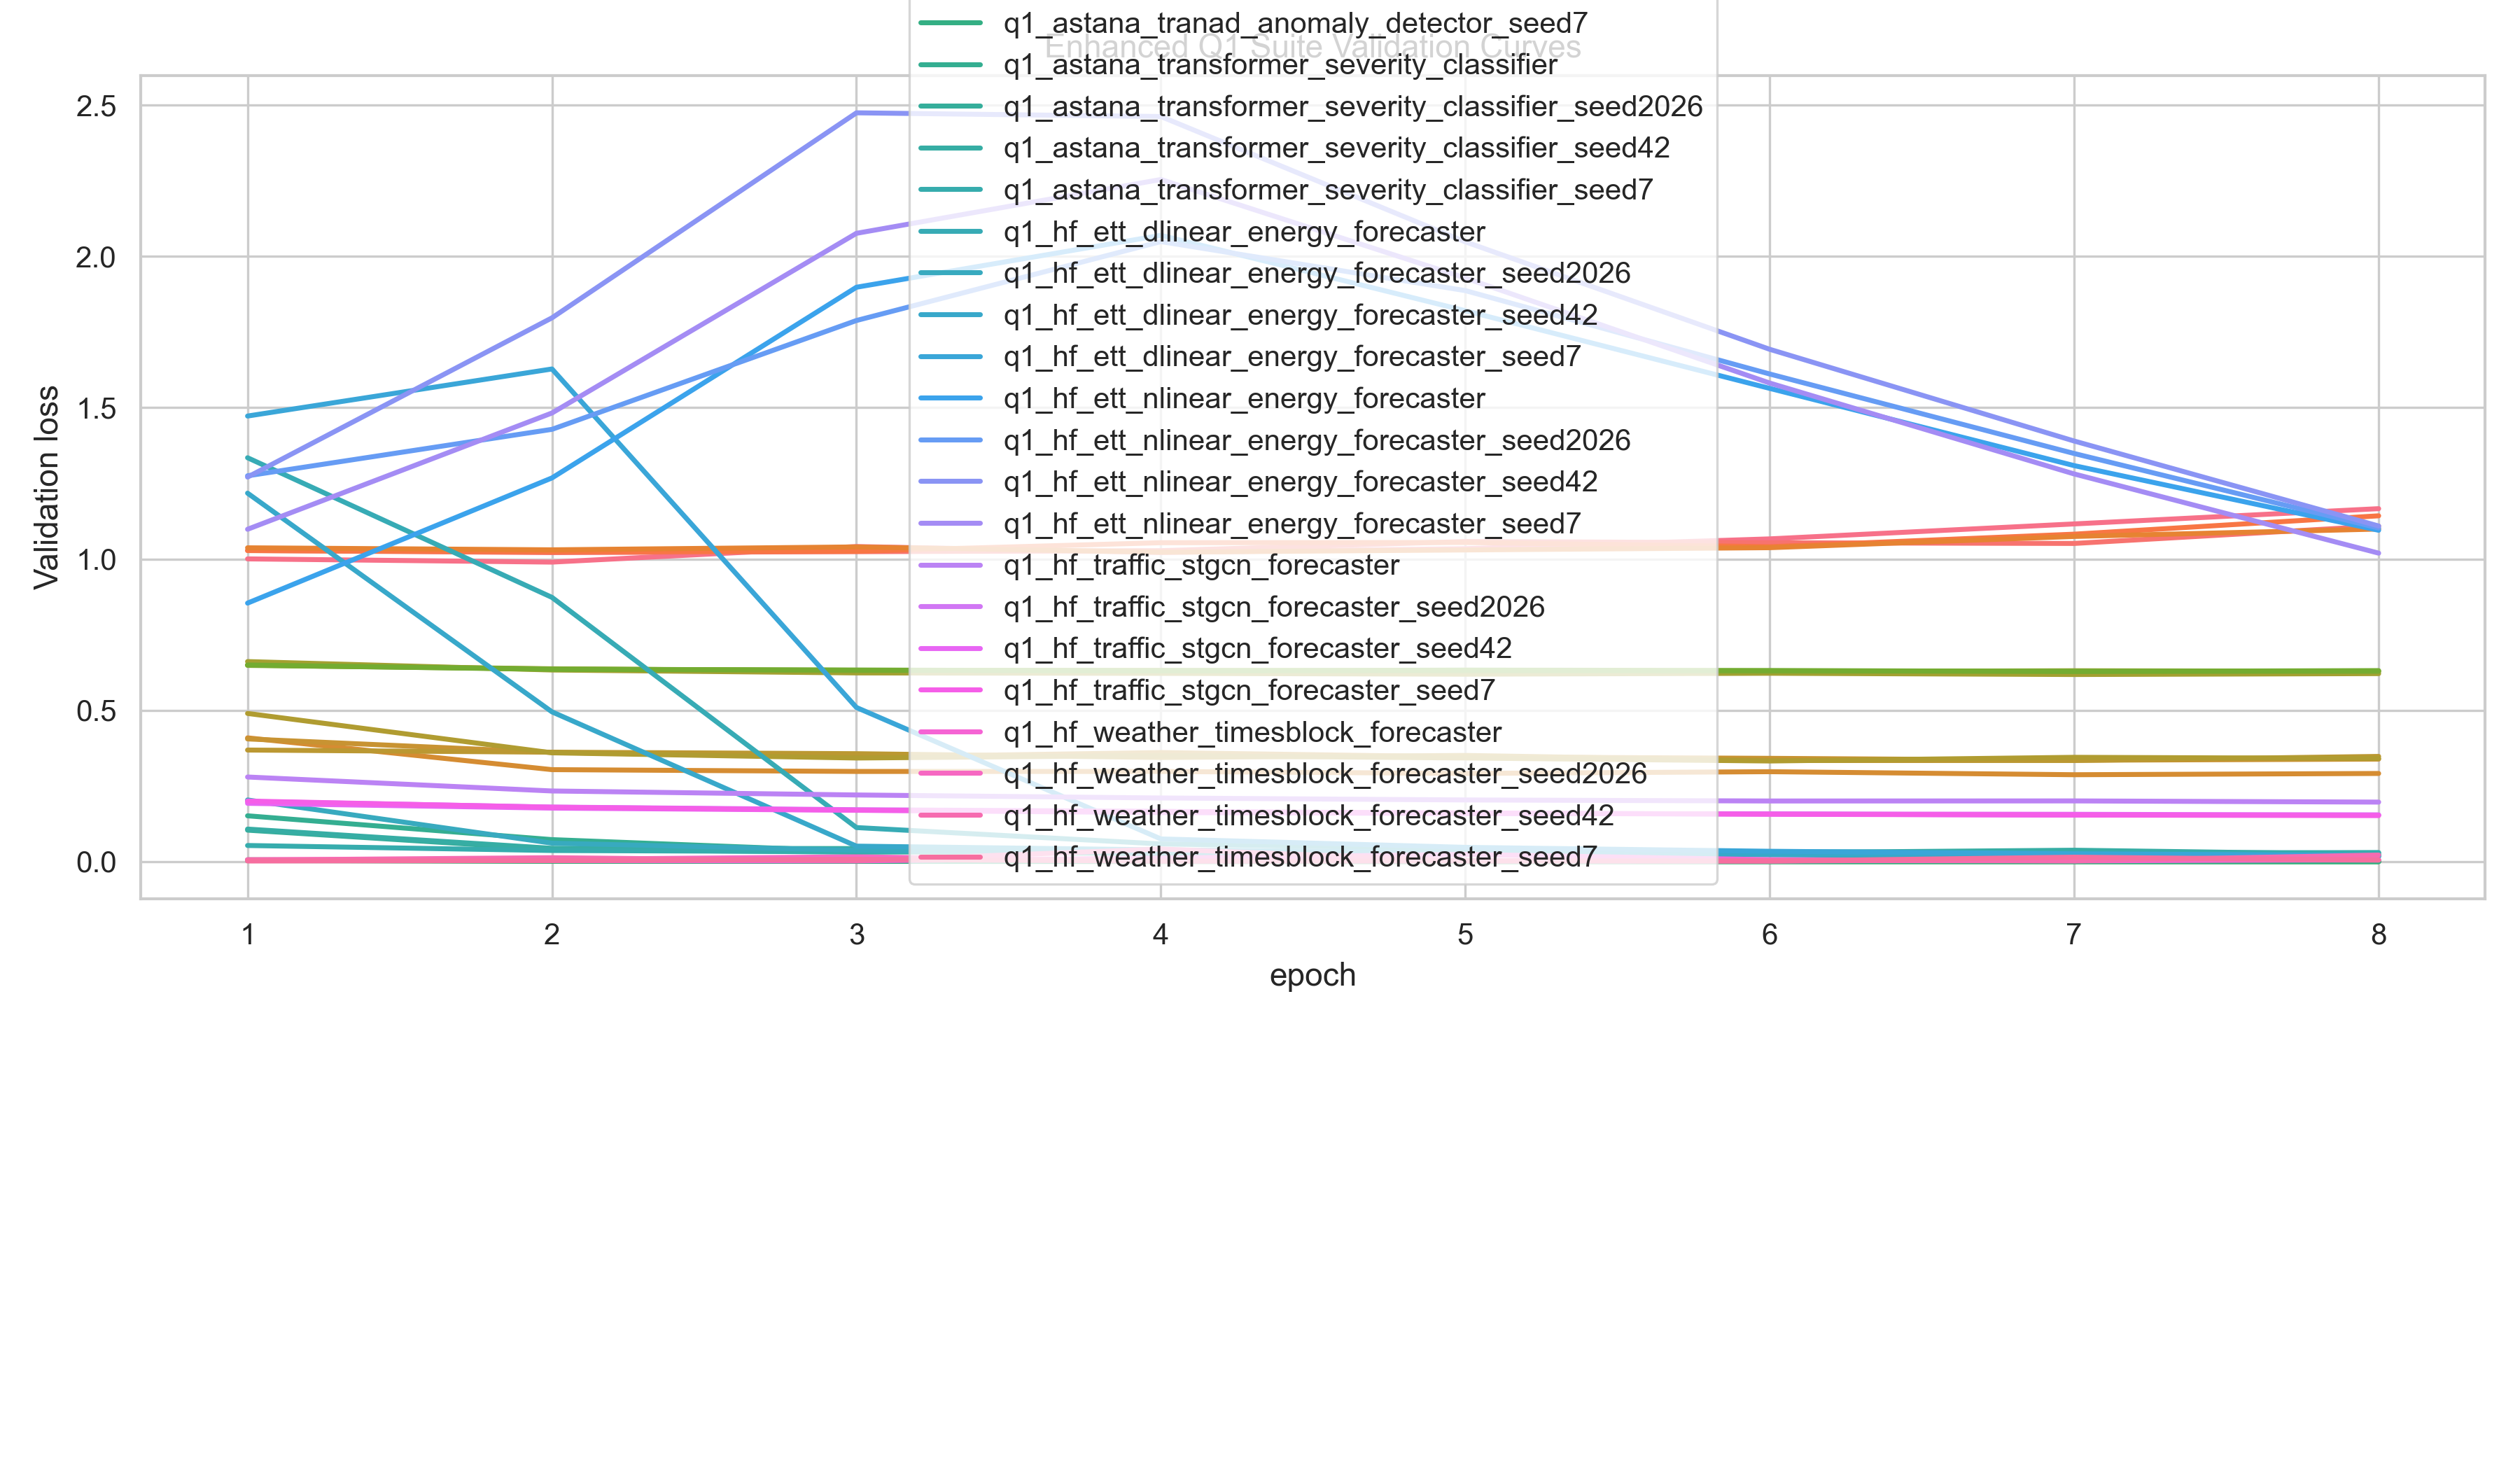
\includegraphics[width=0.85\textwidth]{figures/results/validation_curves_training.png}
  \caption{Validation loss curves during neural model training (representative runs).}
  \label{fig:validation-curves}
\end{figure}

\begin{figure}[H]
  \centering
  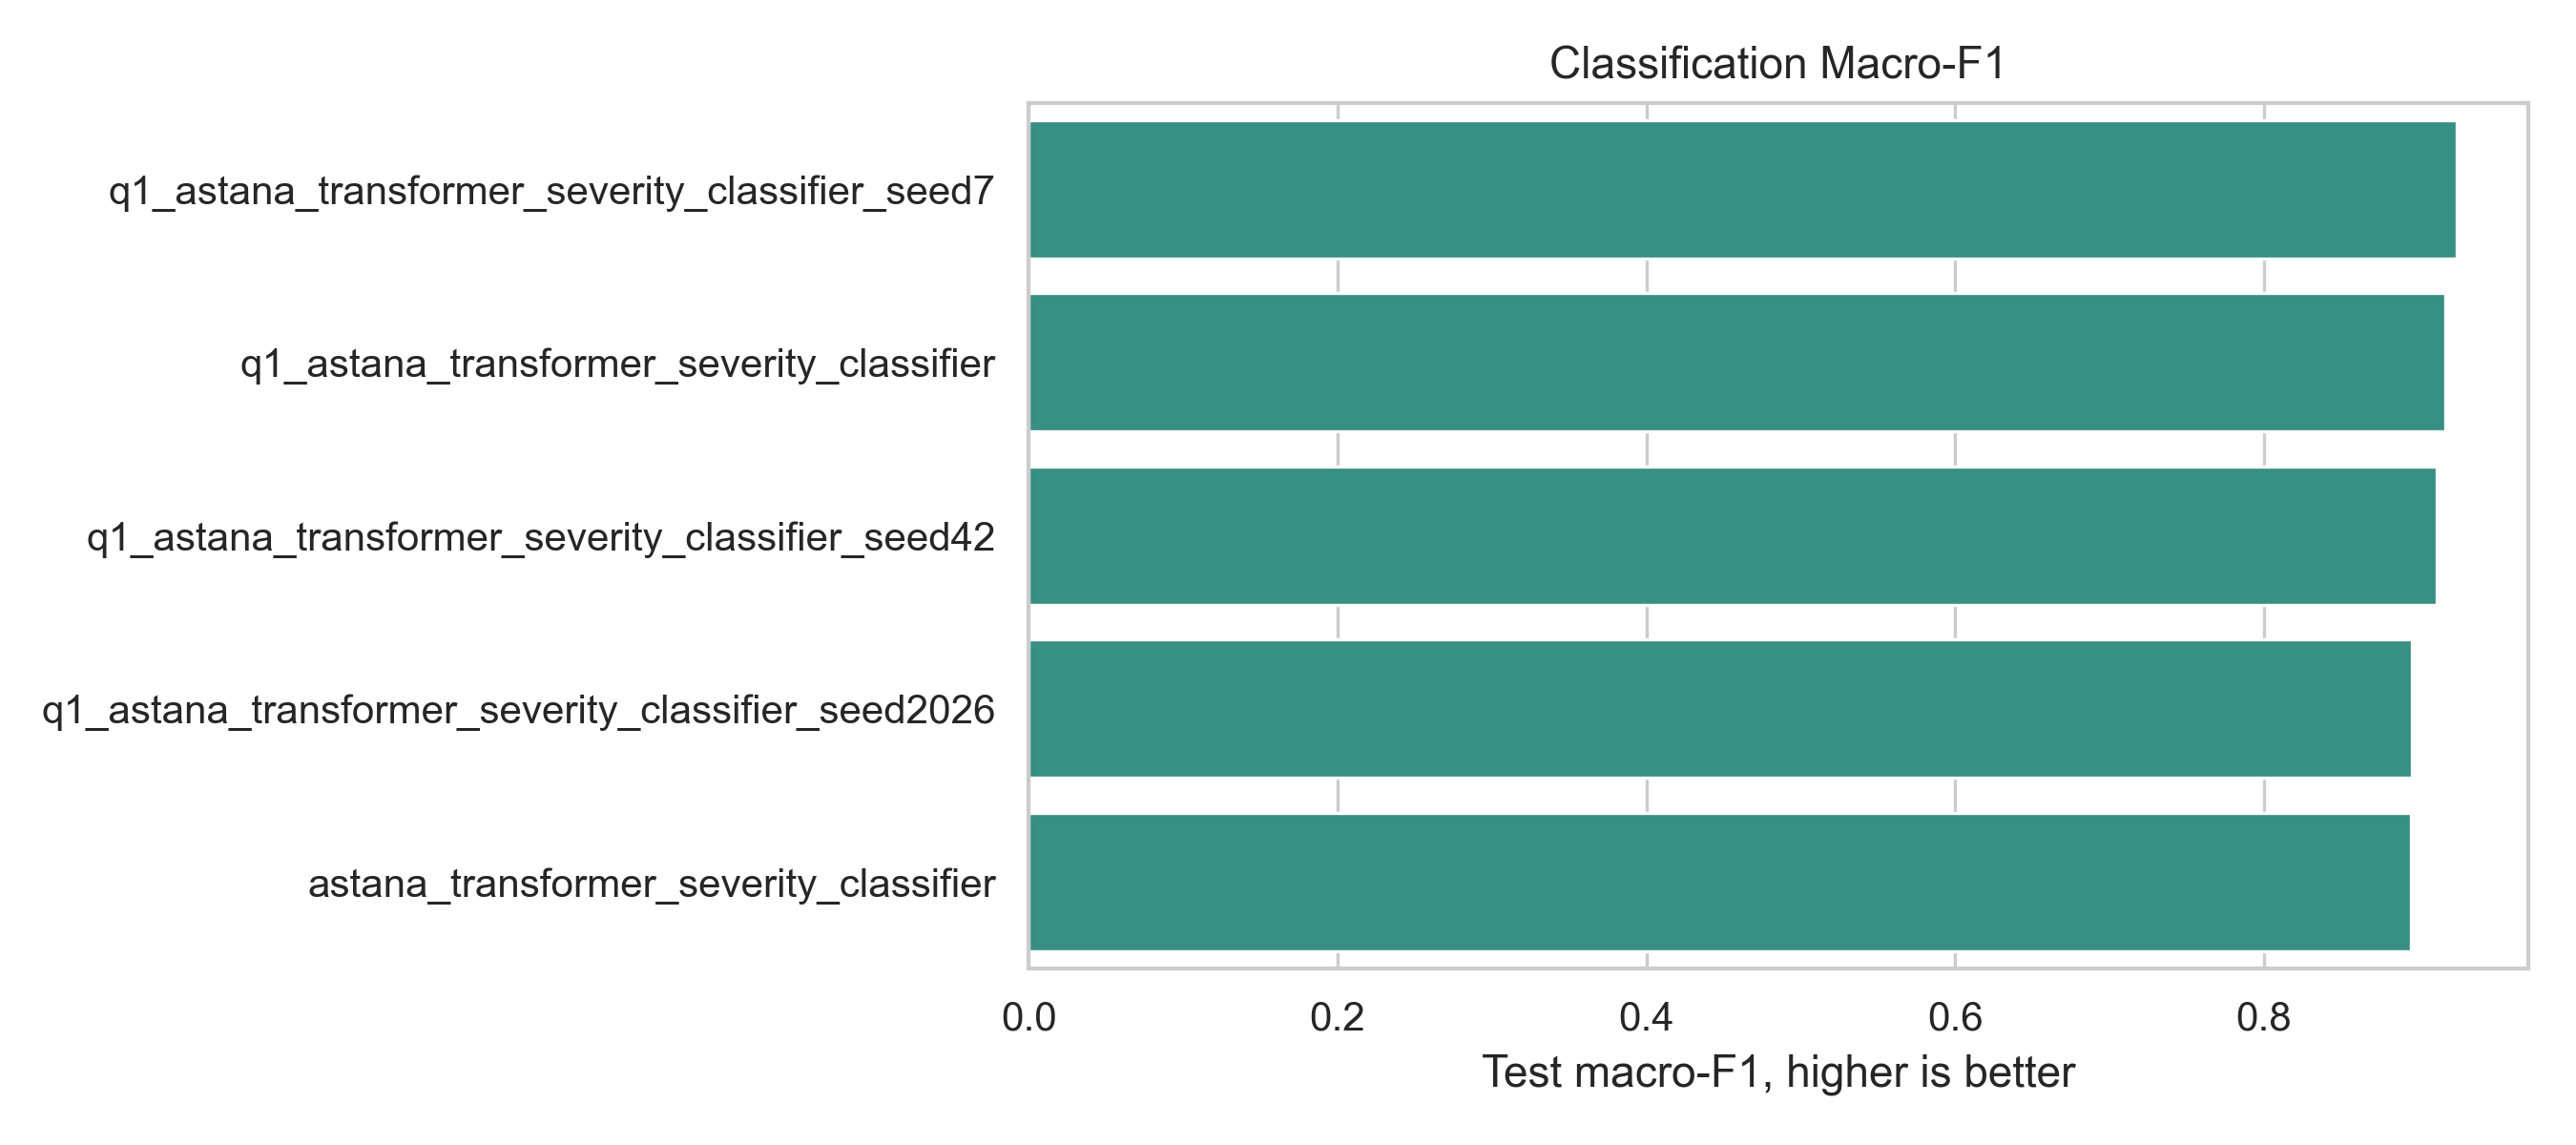
\includegraphics[width=0.78\textwidth]{figures/results/classification_macro_f1.png}
  \caption{Severity classifier macro-F1 compared with classical baselines.}
  \label{fig:neural-classification-f1}
\end{figure}
